\documentclass[12pt,a4paper]{article}
\usepackage[spanish]{babel}
\usepackage[utf8]{inputenc}
\usepackage{graphicx}
\usepackage{graphics}
\usepackage{epsfig}
\usepackage{amsmath}
\usepackage{caption}
\usepackage{algorithm}
\usepackage{algorithmic}
\usepackage{url,hyperref,times}
\usepackage[T1]{fontenc}
\usepackage{color,listings,tikz}
\selectlanguage{spanish}
\usepackage{times}
\usepackage{verbatim,scalefnt,colortbl}
\newtheorem{mydef}{Definición}
\providecommand{\e}[1]{\ensuremath{\times 10^{#1}}}
\DeclareCaptionType{myeq}[][Lista de ecuaciones]
\captionsetup[myeq]{labelformat=empty}

\title{ {\bf Whole genome alignment in high performance computing environments} \\
\it Informe del progreso de trabajo de investigaci\'on} 
\author{ {\bf Julio C\'esar Garc\'ia Vizca\'ino}  \\ 
Departamento de Arquitectura de Computadores y Sistemas Operativos \\ 
Universidad Aut\'onoma de Barcelona\\ 
{\small jcgarcia@aomail.uab.es} 
}
\date{\today}

\begin{document}
\pagestyle{plain}
\pagenumbering{roman}
\maketitle
\pagebreak
{\Huge{\bf Datos del doctorando}}\\
{\Large \\Nombre Completo: Julio César García Vizcaíno\\}
\vspace{0.3cm}
{\Large NIE: Y1497678R\\}
{\Huge{\bf Datos del proyecto de tesis}}\\
\vspace{0.3cm}
{\Large \\Estudio de doctorado: Computación de Altas Prestaciones\\}
\vspace{0.3cm}
{\Large \\Título del proyecto de tesis doctoral: \emph{
Whole genome alignment in high performance computing environments.}\\}
\vspace{0.3cm}
%{\Large \\Palabras claves: Alineamiento de genoma, cadena coincidente,
%datos de secuencia biol\'ogica a gran escala, C\'omputo de altas prestaciones.\\}
%\vspace{0.5cm}
{\Large \\Directores de la tesis: Antonio Espinosa, Juan Carlos Moure.\\}
\vspace{0.3cm}
{\Large \\Línea de investigación: Aplicaciones bioinformáticas.\\}
\vspace{0.3cm}
{\Large \\Rgimen de dedicación: completa.\\}
\vspace{0.3cm}
{\Large \\A\~no de inscripci\'on: 2011.\\}
\vspace{0.3cm}
{\Large \\A\~no previsto para la presentaci\'on de Tesis Doctoral: 2014\\}
\vspace{0.3cm}
{\large \\Firmado\\}
\vspace{2.8cm}
\begin{center}
\begin{tabular}{ c c c }
Director & Director & Estudiante\\
Antonio Espinos & Juan Carlos Moure & Julio C\'esar García Vizcaíno\\
\end{tabular}
\end{center}
\pagebreak
%\cleardoublepage
\pagenumbering{arabic}
\section{Resumen}
\indent
Actualmente la generación de nueva información genómica ha creado la necesidad de almacenar y procesar estos nuevos datos computacionalmente hablando. Una de las tareas en la que nos centramos es el alineamiento de genomas ya que es una tarea computacionalmente intensiva. La información básica de un genoma es el ADN. El ADN es una cadena compuesta por el alfabeto $\sigma={a,c,g,t}$, cada uno de estos elementos es llamado nucleótido. El alineamiento de genomas consiste en encontrar un mapeo de cada posición en un genoma de consulta a su correspondiente positición en el genoma de referencia. Es decir, encontrar las similitudes y diferencias de las cadenas de ADN entre genomas.\\
El alineamiento de genomas es un modelo matemático utilizado por los biólogos para determinar la similitud entre genomas. Un alineamiento involucra tres operaciones básicas:
\begin{itemize}
  \item Coincidencia: los nucleótidos en ambos genomas son iguales.
  \item Discrepancia: los nucleótidos no coinciden en ambos genomas.
  \item Mutaciones: uno o varios cambios de nucleótidos en el genoma:
    \begin{itemize}
      \item Sustitución: un nucleótido es reemplazado por otro.
      \item Inserción: uno o varios nucleótidos se insertan en una posición en el genoma.
      \item Eliminación: uno o varios nucleótidos se borran del genoma.
    \end{itemize}
\end{itemize}
%Los algoritmos utilizados para el alineamiento de genomas presentan una alta demanda computacional debido al tamaño de los datos genómicos.\\
\indent
Existe diferentes algoritmos propuestos para el alineamiento de dos secuencias como \cite{Needleman1970General} y \cite{Waterman}. Estos algoritmos funcionan bien con tamaños de secuencias pequeños como un gen, 20-30kbp\footnote{bp es la únidad básica de medida en las secuencias de ADN y representa la longitud de un nucleótido}. Sin embargo, son ineficaces al alinear genomas enteros. La complejidad computacional y espacial es $O(nm)$, donde $n$ y $m$ son las longitudes de los genomas a alinear. Estos algoritmos tienen problemas de mayores requerimientos de memoria o de tiempos de ejecución inaceptables.\\
\indent
Para grandes secuencias, como el genoma humano (3Gbp), el uso de recursos computacionales pueden ser extremadamente grande y con un largo tiempo de ejecución. Es por ello que han surgido alternativas para reducir el tiempo de ejecución del alineamiento de secuencias. Una de esas alternativas es la utilización de la heurística basada en las coincidencias exactas máximas en las secuencias a alinear. Al encontrar las coincidencias exactas máximas se puede realizar el alineamiento de genomas enteros reduciendo el espacio del alineamiento a las regiones entre las coincidencias exactas máximas.\\
\indent
Formalmente el problema de la búsqueda de coincidencias exactas máximas se define como:
\begin{mydef}
  Dadas dos secuencias (genomas) $R=r_{1}r_{2}\hdots r_{n}$ y $Q=q_{1}q_{2}\hdots q_{m}$, y una longitud mínima $l$, se requiere encontrar todas las ocurrencias de las coincidencias exactas máximas de longitud mínima $l$, entre $R$ y $Q$.
\end{mydef}
Existen diferentes aproximaciones para resolver el problema ver Figura \ref{fig:state}, todas ellas involucran un sacrificio de recursos de cómputo (memoria, procesador).
\begin{figure}[h] 
   \centering 
   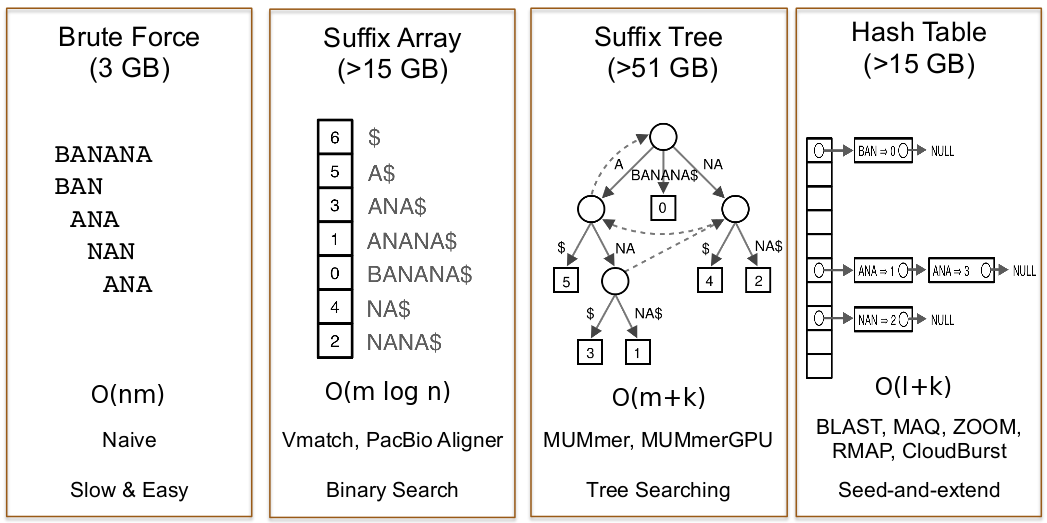
\includegraphics[scale=0.3]{state.png} 
   \caption{Diferentes estructuras de indexación para el problema de la búsqueda de coincidencias exactas máximas para el genoma humano como referencia.} 
   \label{fig:state} 
 \end{figure}
\indent
El árbol de sufijos es una estructura de datos que permite la b\'usqueda de coincidencias exactas de longitud variable en tiempo lineal respecto a la longitud de la secuencia de consulta. Una coincidencia exacta de longitud $w$ ocurre en $r_{i}r_{i+1}\hdots r_{i+l-1}$ y $q_{j}q_{j+1}\hdots q_{j+l-1}$ si y solo si los sufijos $r_{i}r_{i+1}\hdots r_{n}$ y $q_{j}q_{j+1}\hdots q_{m}$ comparten un prefijo común de longitud mínima $l$. La búsqueda de coincidencias máximas exactas en un árbol de sufijos se realiza recorriendo el trayecto que es común a la secuencia de consulta hasta encontrar una discrepancia. Si la búsqueda termina en un nodo hoja, la coincidencia es única en la secuencia de referencia. Verificando el carácter inmediato anterior al inicio de esta coincidencia se puede determinar si es una coincidencia  máxima.\\
\indent
Este problema se presenta en aplicaciones de alineamiento de genomas donde el tama\~no de los genomas son de millones de caracteres y en consecuencia la búsqueda de MEMs es una tarea computacionalmente intensiva. Además, la razón de utilizar un árbol de sufijos radica en que la búsqueda de coincidencias exactas de longitud variable en un árbol de 
sufijos se realiza en tiempo lineal, gracias al uso de los enlaces de sufijos.\\
\indent
En consecuencia se busca \textbf{acelerar la búsqueda eficiente de 
coincidencias exactas y que tenga en cuenta el uso de recursos de cómputo y
memoria en un clúster multicore}. Las consideraciones que se toman en cuenta son:
\begin{itemize}
\item Reducir el número de operaciones en la búsqueda de MEMs: al agilizar la búsqueda se reduce el tiempo utilizado por cada MEM encontrado debido a que los MEMs son dependientes de los datos de entrada.
\item Almacenar genomas de mayor tamaño con la memoria disponible: al utilizar un árbol de sufijos como estructura de indexación el tamaño del árbol se convierte en un problema cuando este no cabe en la memoria disponible. Se hace necesario diseñar estructuras de datos que permitan la indexación de genomas mayores.
\item Reducir los problemas de localidad en el árbol de sufijos: al navegar en un árbol de sufijos puede ocurrir que ocurran fallos de cache.
\end{itemize}
\section{Introducción} 
\subsection{MUM y MEM} 
\indent
La heurística basada en la búsqueda de coincidencias exactas máximas para el alineamiento de genomas requiere de la definición formal de una coincidencia exacta máxima (MEM).\\
\begin{mydef}
  Un MEM (Maximal Exact Match) es una subcadena común a dos
  genomas que es mayor que una longitud mínima específica $d$ de tal manera
  que es máxima, esto es, que no puede ser extendida en ambos extremos sin
  incurrir en una discrepancia. 
\end{mydef}
\indent
Adicionalmente, a partir de la definición de MEM surge el concepto de la coincidencia única maxima (MUM).\\
\begin{mydef}Un MUM (Maximal Unique Match) es una subcadena única común a dos genomas que es mayor que una longitud mínima específica $d$ de tal manera que es máxima, esto es, que no puede ser extendida en ambos extremos sin incurrir en una discrepancia.
\end{mydef}
Identificar las cadenas, $k$, mas grandes en el genoma $Q$ que tienen una coincidencia de longitud $l$ idéntica en el genoma $R$, tiene la siguiente complejidad computacional:
\begin{itemize}
  \item Método simple: $O(nl)$
  \item Usando árbol de sufijos: $O(l+k)$
\end{itemize}
\indent
El objetivo es buscar todas aquellas subcadenas que son comunes a las secuencias de referencia $R$ y consulta $Q$ que son máximas de longitud.\\
\subsection{Árbol de sufijos}
\indent
 Cualquier cadena de referencia de longitud $n$ puede ser descompuesta en $s$ sufijos, ver
 Figura \ref{fig:st}, y estos sufijos pueden almacenarse en un árbol de sufijos.
 Para crear esta estructura de datos se requiere de un tiempo $O(n)$ y para
 buscar una cadena en él requiere de un tiempo $O(l)$ donde $l$ es la longitud
 de la cadena \cite{Gusfield2007Algorithms}. Estas dos propiedades hacen al árbol
 de sufijos una estructura útil para un rango diverso de aplicaciones
 bioinformáticas, incluyendo: alineamiento de genomas \cite{Mummer3}.\\
   \begin{figure}[h] 
   \centering 
   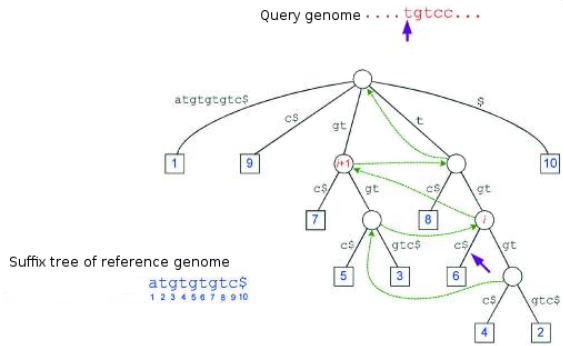
\includegraphics[scale=0.8]{st-mum.png} 
   \caption{Árbol de sufijos para la palabra atgtgtgtc\$.} 
   \label{fig:st} 
 \end{figure}
\indent
La búsqueda de coincidencias exactas máximas en un árbol de sufijos se realiza recorriendo el árbol
con la cadena que se requiere encontrar la coincidencia exacta máxima. Si la coincidencia termina en 
un nodo hoja, la coincidencia exacta máxima es única en la secuencia de referencia. Verificando el 
carácter inmediato anterior al inicio de la posición de la coincidencia es posible determinar si es
máxima.\\
\indent
Por lo tanto es posible identificar todas las coincidencias exactas máximas en tiempo proporcional a
la longitud del genoma de consulta. Es importante resaltar que las coincidencias encontradas no son
necesariamente únicas en el genoma de consulta. Esto se debe a que al recorrer el genoma de consulta, 
las coincidencias encontradas no nos permiten identificar si son únicas ya que no es posible determinar
que coincidencias se encontrarán posteriormente en el genoma de consulta.\\
\indent
En la Figura \ref{fig:st} se muestra como una secuencia de consulta es buscada en el árbol de sufijos. El
árbol representa la secuencia de referencia atgtgtgtc\$. Las hojas representadas en la figura \ref{fig:st} por cuadrados indican la
posición en la que inicia el sufijo. Por ejemplo, la hoja 7 representa el sufijo gtc\$ que inicia en la 
posición 7 de la secuencia de referencia y que está formado por la secuencia de aristas etiquetadas desde la
raíz hasta el nodo hoja 7. En el punto mostrado en la figura, se ha encontrado la coincidencia en la posición $i$,
indicada por la flecha. La coincidencia se extiende a la correspondiente posición en el árbol. En este caso sabemos
que la coincidencia es única en la referencia por que estamos ubicados en un nodo hoja. El número del nodo hoja
nos da la posición de inicio de la coincidencia en la referencia.\\
\indent
Para encontrar la siguiente coincidencia en la cadena de consulta, usamos los enlaces de sufijos, señalados en la Figura \ref{fig:st} por
flechas punteadas. Estos enlaces son construidos para cada nodo interno en el árbol. Un enlace apunta de un nodo
$x$ a un nodo $y$ si el sufijo de la raíz a $y$ es igual al sufijo desde la raíz a $x$ con el primer carácter 
eliminado. Por ejemplo, la cadena del nodo $i$ en la Figura \ref{fig:st} es tgt y del nodo $i+1$ es gt. Esa es la
posición en el árbol correspondiente a la siguiente posición en la secuencia de consulta. Desde el nodo $i$ podemos
continuar la coincidencia bajando en el árbol para determinar que tan grande es la coincidencia puede extenderse. Las 
coincidencias son máximas hacia la derecha cuando se buscan en el árbol de sufijos. Para verificar si son máximas a
la izquierda comparamos los caracteres precedentes en cada cadena. En el ejemplo de la Figura \ref{fig:st}, la
coincidencia inicia en $i+1$ en la cadena de consulta y en el nodo 7 de la cadena del árbol no es máxima a la izquierda
porque el carácter precedente en ambas cadenas es $t$.\\
\indent
El primer algoritmo para la construcción de un árbol de sufijos en tiempo lineal 
y eficiente en espacio fue propuesto en \cite{McCreight:1976:SST:321941.321946}
, y Ukkonen produjo una variante ``on-line'' de ese algoritmo en \cite{Ukkonen1992}. 
La clave para la búsqueda veloz en un árbol de sufijos es que 
hay un camino desde la raíz para cada sufijo del texto. Esto significa que se 
necesitan $l$ comparaciones para encontrar una cadena de longitud $l$.\\
\indent
Otra mejora de implementación necesario para conseguir un tiempo y espacio 
lineal es el uso de enlaces de sufijos. Un enlace de sufijo es un puntero de un 
nodo interno etiquetado $xS$ a otro nodo interno etiquetado $S$, donde $x$ es un 
carácter arbitrario y $S$ es posiblemente una subcadena vacía. Los enlaces de 
sufijos permiten agilizar el recorrido del árbol sin visitar la raíz del árbol 
debido a que apuntan a la siguiente extensión del sufijo. Los enlaces de sufijos 
y la compresión de las etiquetas de las aristas son los requerimientos claves 
para la implementación del árbol de sufijos en $O(n)$.\\
%\indent
%Existen diferentes implementaciones de árboles de sufijos, cada uno con 
%complejidades espaciales diferentes como se muestra en el Cuadro \ref{tab:stmem}.\\
%\begin{table}[h!]  
%\begin{small}
%\begin{center}
%\begin{tabular}{lll}
%Algoritmo & Complejidad espacial & Tamaño \\
%\hline
%McCreight & $O(28n)$ & 81.48GB \\
%\hline
%Ukkonen & $O(26.4n)$ & 76.95GB \\
%\hline
%Kurtz & $O(15.5n)$ & 45.31GB \\
%\hline
%Sadakane\footnote{Compresión de árbol de sufijos} & $O(n\log|\Sigma|)$ & 8.8GB \\
%\hline
%TRELLIS \cite{Phoophakdee2007} & $O(24.6n)$ & 71.6GB \\
%\hline
%TDD \cite{Barsky2010} & $O(18.5n)$ & 54GB \\
%\end{tabular}
%\end{center}
%\end{small}
%\caption{Algoritmos de creación de árboles de sufijos y su uso de memoria al
%almacenar el genoma humano (n=2.91Gbp).}
%\label{tab:stmem}
%\end{table}
%\\ \indent
%Los árboles de sufijos son dependientes del alfabeto, $\Sigma$, el tamaño 
%del alfabeto, $|\Sigma|$, afecta los tiempos de creación y búsqueda de 
%cadenas en el árbol, $C$, para una cadena de referencia de longitud $n$. 
%Estrictamente hablando:
%    \begin{itemize} 
%      \item Requerimiento de espacio: $O(n)$ 
%      \item Tiempo de creación: $min (O(n\log n), O(n\log |\Sigma|))$ 
%      \item Tiempo de búsqueda: $min (O(|C|\log n), O(|C|\log |\Sigma|))$ 
%    \end{itemize}
%\indent
\subsection{Definición del problema a resolver}
\indent
El problema de la búsqueda de las coincidencias exactas máximas de una longitud mínima ha sido identificado en varias aplicaciones, entre ellas MUMmer \cite{Mummer3}. Aunque el algoritmo de MUMmer realiza la búsqueda de coincidencias exactas máximas, los requerimientos de recursos de cómputo aún son altos debido al tamaño de los datos de entrada.\\
\indent
%Se ha realizado un experimento para comparar las prestaciones de la búsqueda de
%coincidencias exactas máximas utilizando un árbol de sufijos. En el Cuadro 
%\ref{tab:buscar} se muestra el tiempo de procesamiento de búsqueda 
%para coincidencias de tamaño mínimo $L$, utilizando el árbol de sufijos. El tiempo 
%de cómputo invertido en la búsqueda involucra la operación individual de cadenas de longitud mínima $L$ hasta la longitud de la cadena máxima de coincidencia. \\
%\begin{table}[ h!] 
%  \begin{small}
%    \begin{center}
%      \begin{tabular}{lllll}
%        Estructura & L [bp] & Cantidad  & Búsqueda [s] & Uso de\\
%        & & de búsquedas & & memoria [MB] \\
%        \hline
%        Árbol de sufijos & 20 & 344,46\e{6}  & 1679,2 & 483 \\
%        %\hline
%        %Arreglo de sufijos & 20 & 344,46\e{6}  & 5885,7 & 320\\
%        \hline
%      \end{tabular}
%    \end{center}
%  \end{small}
%  \caption{Búsqueda coincidencias exactas para una cadena de referencia de 
%  29,38Mbp y una cadena de consulta de 29,69Mbp}
%  \label{tab:buscar}
%\end{table}
%\indent
%El tiempo de búsqueda del Cuadro \ref{tab:buscar} para cadenas de tamaño de 30Mbp
%es relativamente alto debido a que involucra realizar millones de búsquedas en
%serie. La cantidad de operaciones de búsqueda que se realizan son 11 veces la 
%longitud de las cadenas de referencia y consulta. En consecuencia, la búsqueda 
%de coincidencias exactas máximas es una operación computacionalmente intensiva. 
%La razón de este uso intensivo de cómputo se debe a la cantidad de operaciones de búsqueda
%y a los accesos aleatorios en memoria al hacer cada operación de búsqueda.\\
%\indent
%Al aumentar la longitud de las cadenas de referencia y consulta por un factor de 10, 
%los tiempos de búsqueda se incrementan linealmente por un factor de 10, el uso de 
%memoria aumenta aproximadamente 8 veces y la cantidad de búsquedas a realizar se
%multiplica \e{3} veces, como se observa en el Cuadro \ref{tab:buscar2}.\\
%\begin{table}[ h! ]
%  \begin{small}
%    \begin{center}
%      \begin{tabular}{lllll}
%        Estructura & L [bp] & Cantidad  & Búsqueda [s] & Uso de\\
%        & & de búsquedas & & memoria [MB] \\
%        \hline
%        Árbol de sufijos & 20 & 3,78\e{9}  & 13013,5 & 3890 \\
%        %\hline
%        %Arreglo de sufijos & 20 & 3,78\e{9}  & 45616,2 & 2293\\
%        \hline
%      \end{tabular}
%    \end{center}
%  \end{small}
%  \caption{Búsqueda coincidencias exactas para una cadena de referencia de 
%  227,69Mbp y una cadena de consulta de 238,62Mbp}
%  \label{tab:buscar2}
%\end{table} 
%\indent
Si la longitud de los genomas son muy grandes, ver Cuadro \ref{tab:buscar3}, 
la cantidad de búsquedas aumentan, el tiempo de búsqueda
crece linealmente y el uso de memoria se convierte en un problema a resolver si
se considera la disponibilidad finita de memoria en la mayoría de sistemas de
cómputo personales.\\
\begin{table}[ h!]
  \begin{small}
    \begin{center}
      \begin{tabular}{lllll}
        Estructura & L [bp\footnote{Par base, unidad básica de medición de nucleótidos en una secuencia de ADN.}] & Cantidad  & Búsqueda [s] & Uso de\\
        & & de búsquedas & & memoria [MB]\\
        \hline
        Árbol de sufijos & 20 & 9,87\e{18}  & 169189,4 & 48665,12\\
        \hline
        %Arreglo de sufijos & 20 & 9,87\e{18}  & 593019,3 & 32241,9\\
        %\hline
      \end{tabular}
    \end{center}
  \end{small}
  \caption{Búsqueda coincidencias exactas para una cadena de referencia de 
  2960,21Mbp y una cadena de consulta de 2716,96Mbp}
  \label{tab:buscar3}
\end{table}
\indent
De acuerdo a los datos del Cuadrs \ref{tab:buscar3} se hace necesario la búsqueda de alternativas que 
permitan llevar a cabo la búsqueda de manera eficiente. El uso de HPC nos permitiría
resolver los problemas de escalabilidad (tiempo de búsqueda, uso de memoria) cuando 
se tienen cadenas muy grandes, como el genoma humano.\\
%\subsection*{Problema} 
%\indent
%La búsqueda de coincidencias exactas máximas es un problema computacionalmente
%intensivo. Dadas una cadena de referencia $R$ de longitud $n$ y una cadena de consulta 
%$Q$ de longitud $m$, encontrar todas las coincidencias de longitud mínima $l$ de $Q$
%en la cadena de referencia $R$ implica recorrer la cadena de consulta $Q$ para $todas$
%sus subcadenas. Para cada subcadena se determina la posición o posiciones en donde 
%existe una coincidencia, de longitud mínima $l$, entre la subcadena y la cadena de 
%referencia $R$. La posición de la subcadena en $Q$ es determinada.\\
%\indent
%En la Figura \ref{fig:problema} se muestra gráficamente el problema de la búsqueda
%de coincidencias exactas máximas.
%\begin{figure}[h]
%\begin{center}
%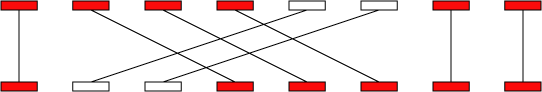
\includegraphics[scale=0.5]{gaps.png}
%\caption{Problema de la búsqueda de coincidencias exactas máximas.}
%\label{fig:problema}
%\end{center}
%\end{figure}
%\\ \indent El total de búsquedas, indicado en los Cuadros \ref{tab:buscar} y \ref{tab:buscar2} 
%a realizar está determinada por la fórmula \ref{eq:operaciones}.
%\begin{equation}
%  \sum_{i=0}^{i\le m}{\frac{n}{L+i}}
%  \label{eq:operaciones}
%\end{equation}
%Realizar una búsqueda de coincidencia exacta de longitud fija es sencilla 
%computacionalmente hablando. Pero al realizar una búsqueda de coincidencia exacta de 
%longitud variable ocurren los siguientes problemas:
%\begin{itemize}
%  \item Acceso aleatorio a la cadena indexada de referencia $R$: el conjunto de coincidencias
%    podría estar en posiciones de la cadena $R$ distantes.
%  \item Longitud variable de la cadena a buscar: la búsqueda a realizar se incrementa
%    con la longitud de la cadena.
%  \item Uso de memoria: para poder buscar una coincidencia se requiere volcar la 
%    cadena de referencia $R$ en memoria. Dependiendo del método utilizado la 
%    cantidad de memoria se podría incrementar e incluso agotar la memoria disponible.
%    Adicionalmente el tiempo de búsqueda se incrementará, como se observa en el 
%    Cuadro \ref{tab:buscar3},debido al acceso a disco cuando no se tiene toda la 
%    cantidad de memoria necesaria.
%\end{itemize}
%Para resolver este problema de forma distribuida existen diferentes estrategias. La 
%solución mas obvia es realizar una división de las cadenas de referencia y
%de consulta, ver Figura \ref{fig:para}.
%\begin{figure}[h]
%\begin{center}
%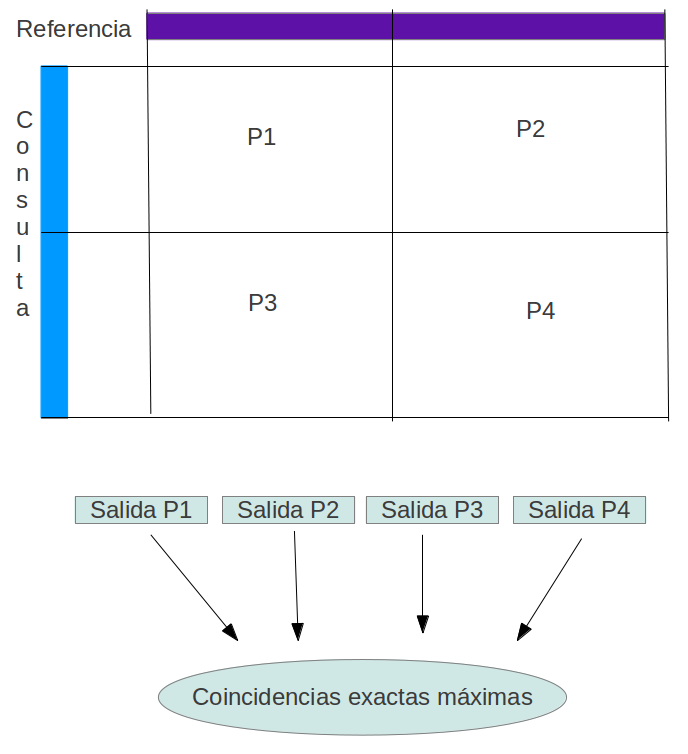
\includegraphics[scale=0.3]{naive.png}
%\caption{Solución obvia de paralelización de búsqueda de coincidencias exactas máximas.}
%\label{fig:para}
%\end{center}
%\end{figure}
%\\Esta técnica ocasiona que exista una fase de procesamiento posterior a la búsqueda de 
%coincidencias exactas máximas en cada segmento de la cadena procesada, para determinar
%las coincidencias máximas de forma global. Adicionalmente, puede haber pérdidas de 
%coincidencias máximas exactas y coincidencias máximas que solo son válidas dentro del 
%segmento evaluado y no de manera global.\\
En consecuencia, para resolver este problema se utiliza alguna estructura de datos que 
permita realizar una búsqueda distribuida de coincidencias exactas máximas de forma ágil 
en la cadena entera. Los árboles de sufijos permiten hacer 
búsquedas con complejidad $O(m+k)$, donde $m$ es el 
tamaño de la cadena a buscar y $k$ es el número de ocurrencias.\\
En resumen la búsqueda de coincidencias exactas máximas en una cadena, como el 
genoma humano, es un problema computacionalmente intensivo que es posible 
resolverse con estructuras de datos como el árbol de sufijos. 
%Sin embargo como se 
%muestra en el Cuadro \ref{tab:estructuras} se reseña las características de cada solución propuesta.\\
%\begin{table}[hc]   
%\begin{small}
%\begin{center}
%\begin{tabular}{llllll}
%Estructura de datos & Memoria & Búsqueda & Ventaja & Desventaja\\
%\hline
%Arreglo de sufijos & $O(10n)$  & $O(m\log n)$, & Eficiente en & Tiempo de búsqueda 
%en  \\ 
%& & $m$ es el tamaño de & uso de espacio.& de coincidencias exactas \\
%& & la cadena a buscar.& inaceptable.\\
%\hline
%Árbol de sufijos & $O(15.5n)$ & $O(m+k)$, & Búsqueda de   & Incremento en \\
%&  &  $m$ es el tamaño de & de coincidencia de & el tiempo de \\ 
%&  & la cadena buscar & cadenas de & búsqueda. \\
%&  &y $k$ el número de ocurrencias. & longitud variable.&\\
%\end{tabular}
%\end{center}
%\end{small}
%\caption{Estructuras de datos para la búsqueda de coincidencia exacta de cadenas.}
%\label{tab:estructuras}
%\end{table}
\indent
Independientemente de la estructura de datos utilizada, lo que se desea es poder
realizar búsquedas de coincidencias exactas a esa estructura de manera eficiente. 
Una de las consultas en que se requiere realizar rápidamente, para el alineamiento 
de genomas, es la búsqueda exacta de coincidencias máximas. 
\section{Estado de la investigación}
\subsection{Paralelización a nivel de datos: alineamiento de genomas}
\indent
La versión secuencial del algoritmo de MUMmer\footnote{Aplicación para el alineamiento de genomas con más de 700 referencias en artículos de investigación.}, requiere mayores recursos de cómputo conforme los genomas a alinear son de longitudes mayores. Un primer problema es cuando la referencia a indexar mediante el árbol de sufijos resulta en un árbol de mayor tamaño a la memoria disponible. El segundo problema es el tiempo empleado para procesar un genoma de consulta.\\
\indent
Es por ello que se realizó una evaluación de la viabilidad de utilizar la t\'ecnica de paralelización de datos en el alineamiento de genomas. Específicamente se evalúa que t\'ecnica de paralelización es mejor: dividir el genoma de referencia o dividir el genoma de consulta. En la figura \ref{fig:algo} se muestra la propuesta evaluada de paralelización a nivel de datos. La paralelización involucra que se realice una división del genoma con un tamaño fijo y una área de solapamiento. El tamaño del bloque es determinado por el número de instancias de ejecución que se tendrán y el solapamiento es utilizado para evitar perder alguna coincidencia debido a la división del genoma. Una vez hecha la división se procede a ejecutar la búsqueda de coincidencias exactas máximas. Al realizar la búsqueda de MEMs se tiene un conjunto de listas parciales de MEMs que se mezclan para obtener la lista global de MEMs que debe ser la misma a una ejecución serie.\\
   \begin{figure}[h] 
   \centering 
   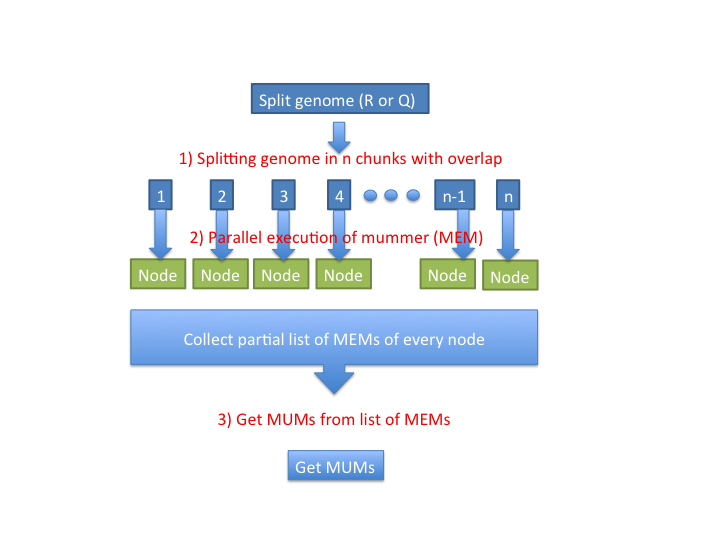
\includegraphics[scale=0.4]{algorithm.png} 
   \caption{Paralelización del alineamiento de genomas.} 
   \label{fig:algo} 
 \end{figure}
\indent
En las figuras \ref{fig:ecoli} y \ref{fig:hspan} se muestran los resultados de la paralelización del alineamiento de genomas reseñado en la figure \ref{fig:algo}. El problema que surge al realizar este tipo de paralelización es en la fase final de obtener la lista global de MEms. Esto es, se requiere contar con un algoritmo que permita descartar aquellos MEMs que están contenidos por otro MEM de mayor tamaño y que no son posible eliminar en la fase previa debido a que se requiere evaluar el resto de los MEMs.\\
   \begin{figure}[h] 
   \centering 
   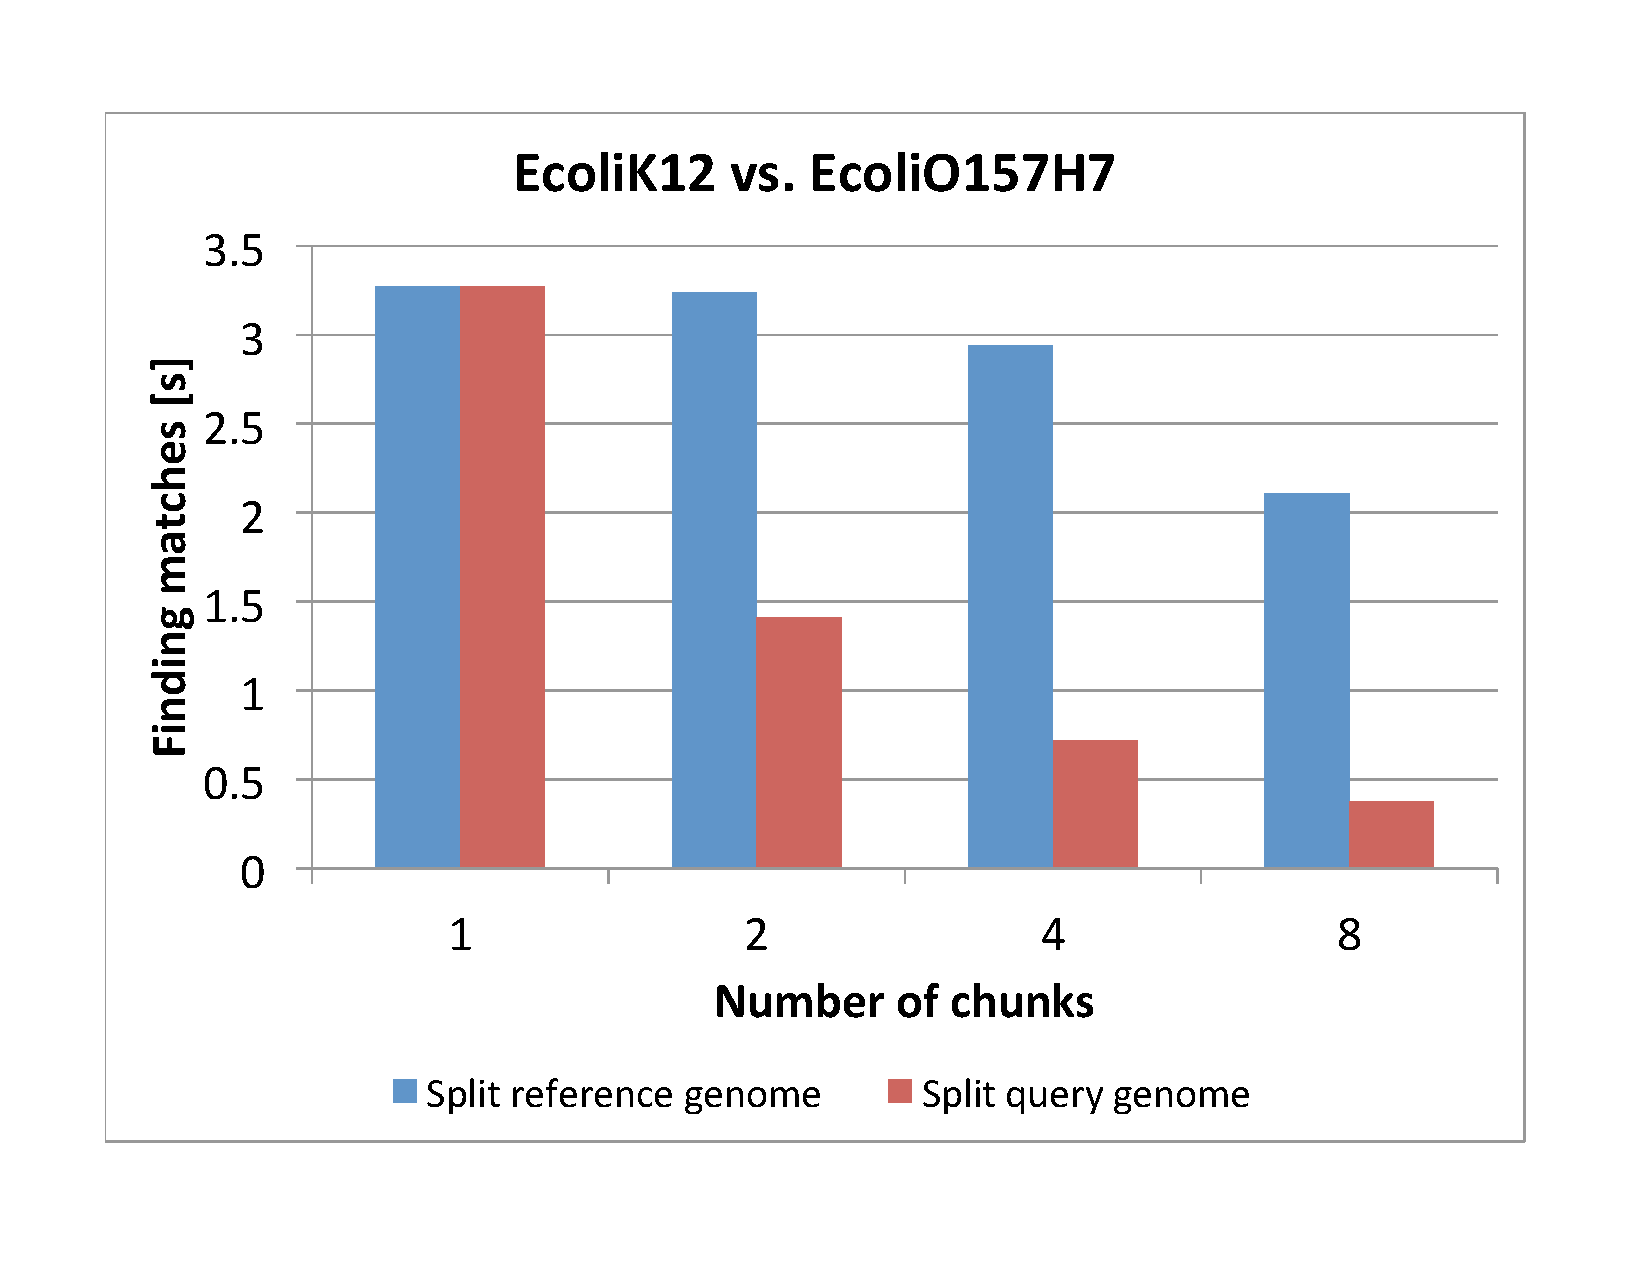
\includegraphics[scale=0.4]{ecoli2012.pdf} 
   \caption{Paralelización del alineamiento del genoma Ecoli con longitud de 5,4Mbp.} 
   \label{fig:ecoli} 
 \end{figure}
   \begin{figure}[h] 
   \centering 
   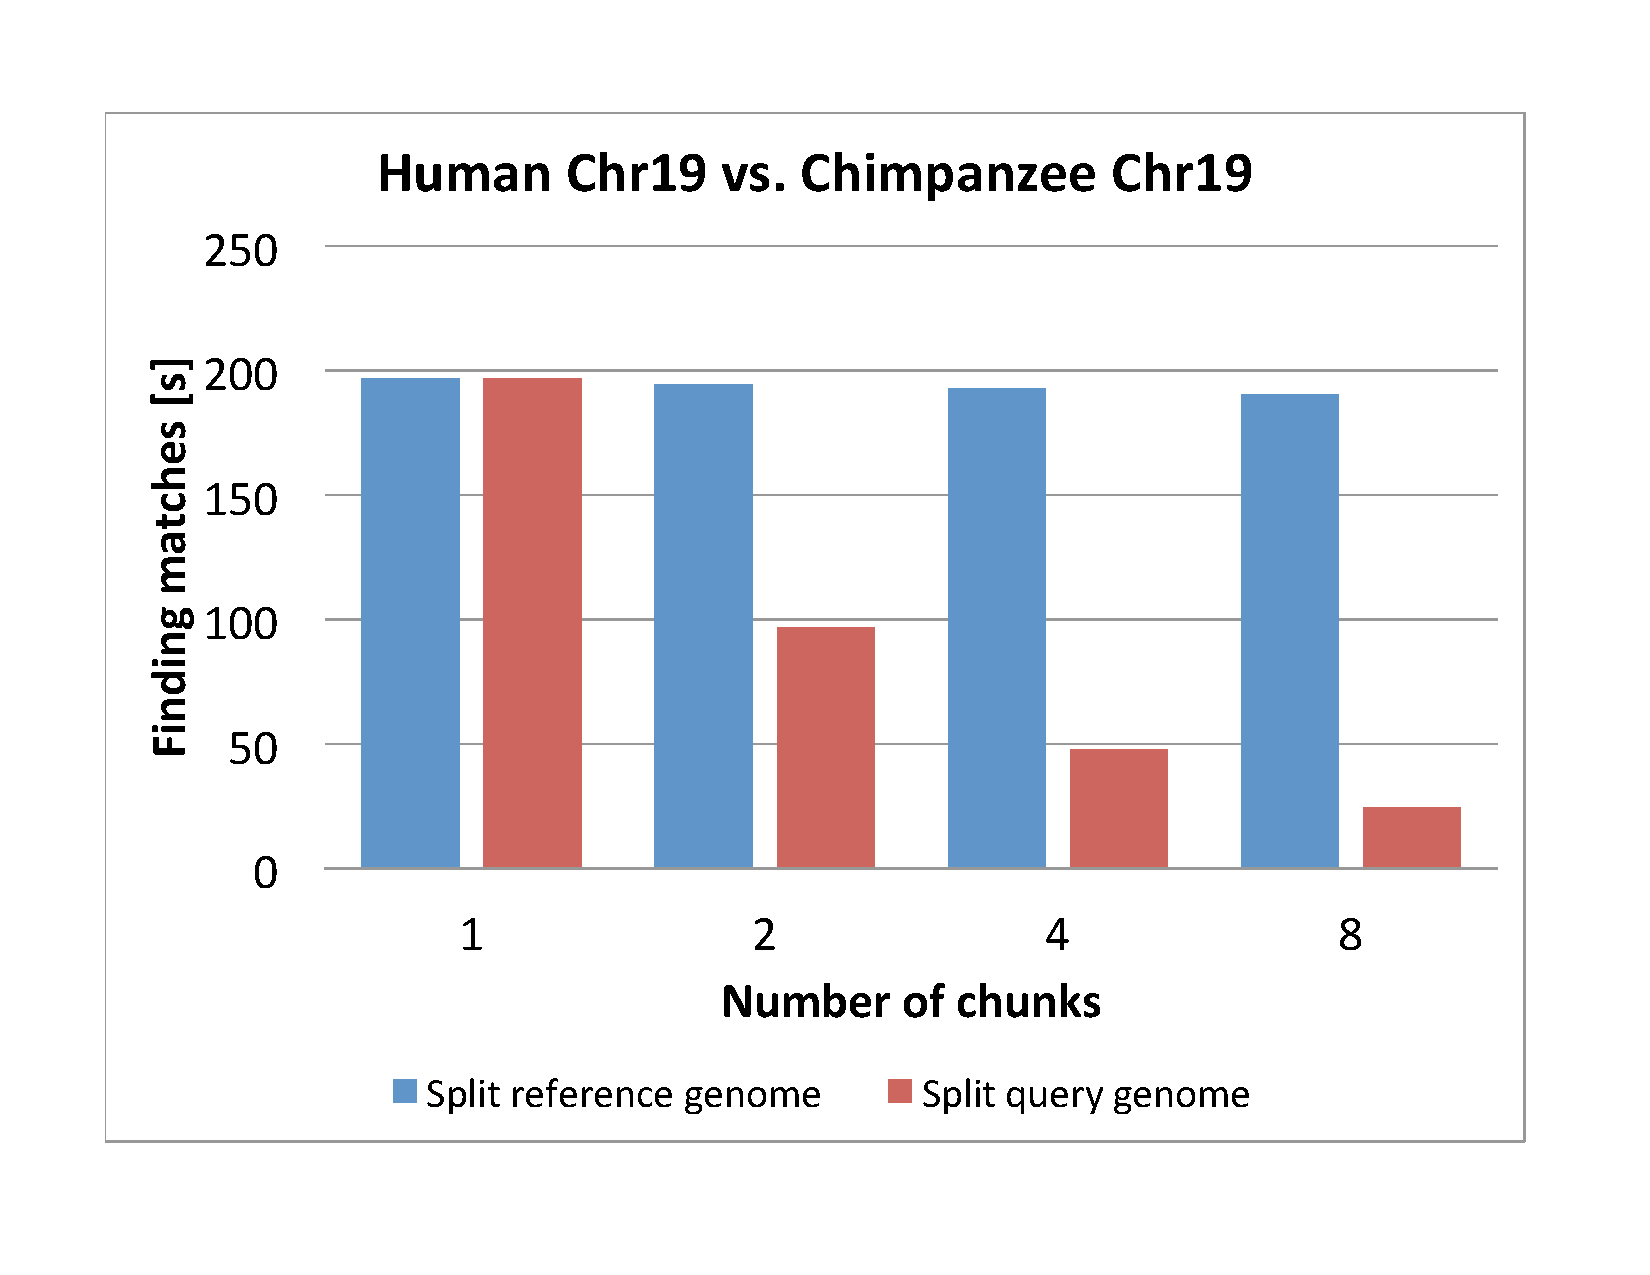
\includegraphics[scale=0.4]{hspan.pdf} 
   \caption{Paralelización del alineamiento del cromosoma 19 del homo sapiens y el chimpanc\'e con longitud de 59Mbp.} 
   \label{fig:hspan} 
 \end{figure}
\indent
Una primera solución es evaluar para cada MEM si está cubierto por un MEM mayor en toda la lista. Esta solución simple ayuda debido a que tiene una complejidad $O(g^2)$ donde $g$ es la cantidad total de MEMs encontrados, es por ello que se necesita un algoritmo que permita efizcamente descartar aquellos MEMs que están repetidos y/o contenidos por otro MEM.\\
\indent
La propuesta para un nuevo algoritmo de mezcla final de MEMs toma en cuenta el principio de que basta con evaluar solo aquella región que contiene al MEM que estamos evaluando. De esa manera es posible disminuir la complejidad del algoritmo y el tiempo de cómputo total de la paralelización no sería penalizado por la última fase. El algoritmos es descrito a continuación:
\begin{algorithmic}
  \STATE Conjunto de MEMs parciales: A.
  \STATE Quicksort de MEMs parciales por la posición en la consulta.
  \FOR{$i=0$ a $N$}
      \STATE $A[i].Good=TRUE$
  \ENDFOR
  \FOR{$i=0$ a $i<N-1$}
      \IF{$!A[i].Good$}
          \STATE Continuar.
      \ENDIF
      \STATE $i\_diag=A[i].Q-A[i].R$
      \STATE $i\_fin=A[i].Q+A[i].Len$
      \FOR{$j=i+1;j<N\&\&A[j].Q\le i\_fin;j++$}
          \IF{$!A[j].Good$}
              \STATE Continuar.
          \ENDIF
          \STATE $j\_diag=A[j].Q-A[j].R$
          \IF{$i\_diag==j\_diag$}
              \STATE $j\_extent=A[j].Len+A[j].Q-A[i].Q$
              \IF{$j\_extent>A[i].Len$}
                  \STATE $A[i].Len=j\_extent$
                  \STATE $i\_end=A[i].Q+j\_extent$
              \ENDIF
              \STATE $A[j].Good=FALSE$
          \ELSIF{$A[i].R==A[j].R$}
              \STATE $olap=A[i].Q+A[i].Len-A[j].Q$
              \IF{$A[i].Len<A[j].Len$}
                  \IF{$olap\ge A[i].Len/2$}
                      \STATE $A[i].Good=FALSE$
                      \STATE Romper.
                  \ENDIF
              \ELSIF{$A[j].Len<A[i].Len$}
                  \IF{$olap\ge A[j].Len/2$}
                      \STATE $A[j].Good=FALSE$
                  \ENDIF
              \ELSE
                  \IF{$olap\ge A[i].Len/2$}
                      \STATE $A[j].Tentative=TRUE$
                      \IF{$A[i].Tentative$}
                          \STATE $A[i].Good=FALSE$
                          \STATE Romper.
                      \ENDIF
                  \ENDIF
              \ENDIF
          \ELSIF{$A[i].Q==A[j].Q$}
              \STATE $olap=A[i].R+A[i].Len-A[j].R$
              \IF{$A[i].Len<A[j].Len$}
                  \IF{$olap\ge A[i].Len/2$}
                      \STATE $A[i].Good=FALSE$
                      \STATE Romper.
                  \ENDIF
              \ELSIF{$A[j].Len<A[i].Len$}
                  \IF{$olap\ge A[j].Len/2$}
                      \STATE $A[j].Good=FALSE$
                  \ENDIF
              \ELSE
                  \IF{$olap\ge A[i].Len/2$}
                      \STATE $A[j].Tentative=TRUE$
                      \IF{$A[i].Tentative$}
                          \STATE $A[i].Good=FALSE$
                          \STATE Romper.
                      \ENDIF
                  \ENDIF
              \ENDIF
          \ENDIF
      \ENDFOR
  \ENDFOR
  \FOR{$i=j=0;i<N;i++$}
      \IF{$A[i].Good$}
          \IF{$i\ne j$}
              \STATE $A[j]=A[i]$
          \ENDIF
          \STATE $j++$
      \ENDIF
  \ENDFOR
  \STATE $N=j$
  \FOR{$i=0;I<N;i++$}
      \STATE $A[i].Good=FALSE$
  \ENDFOR
\end{algorithmic}
\indent
La complejidad del algoritmo descrito en el peor de los casos es $O(g)$ donde $g$ es el tamaño de la lista total de MEMs parciales, en el mejor de los casos es $O(g)$. Para el genoma Ecoli de longitud 5,4Mbp en donde se buscaron MEMs de longitud mínima de 20, la figura \ref{fig:ecoliFind} muestra el tiempo de cómputo utilizado en la fase de búsqueda de MEMs, en las figuras \ref{fig:ecoliMEMR} y \ref{fig:ecoliMEMQ} se muestra el tiempo utilizado en la fase de obtención de la lista de MEMs global.\\
   \begin{figure}[h] 
   \centering 
   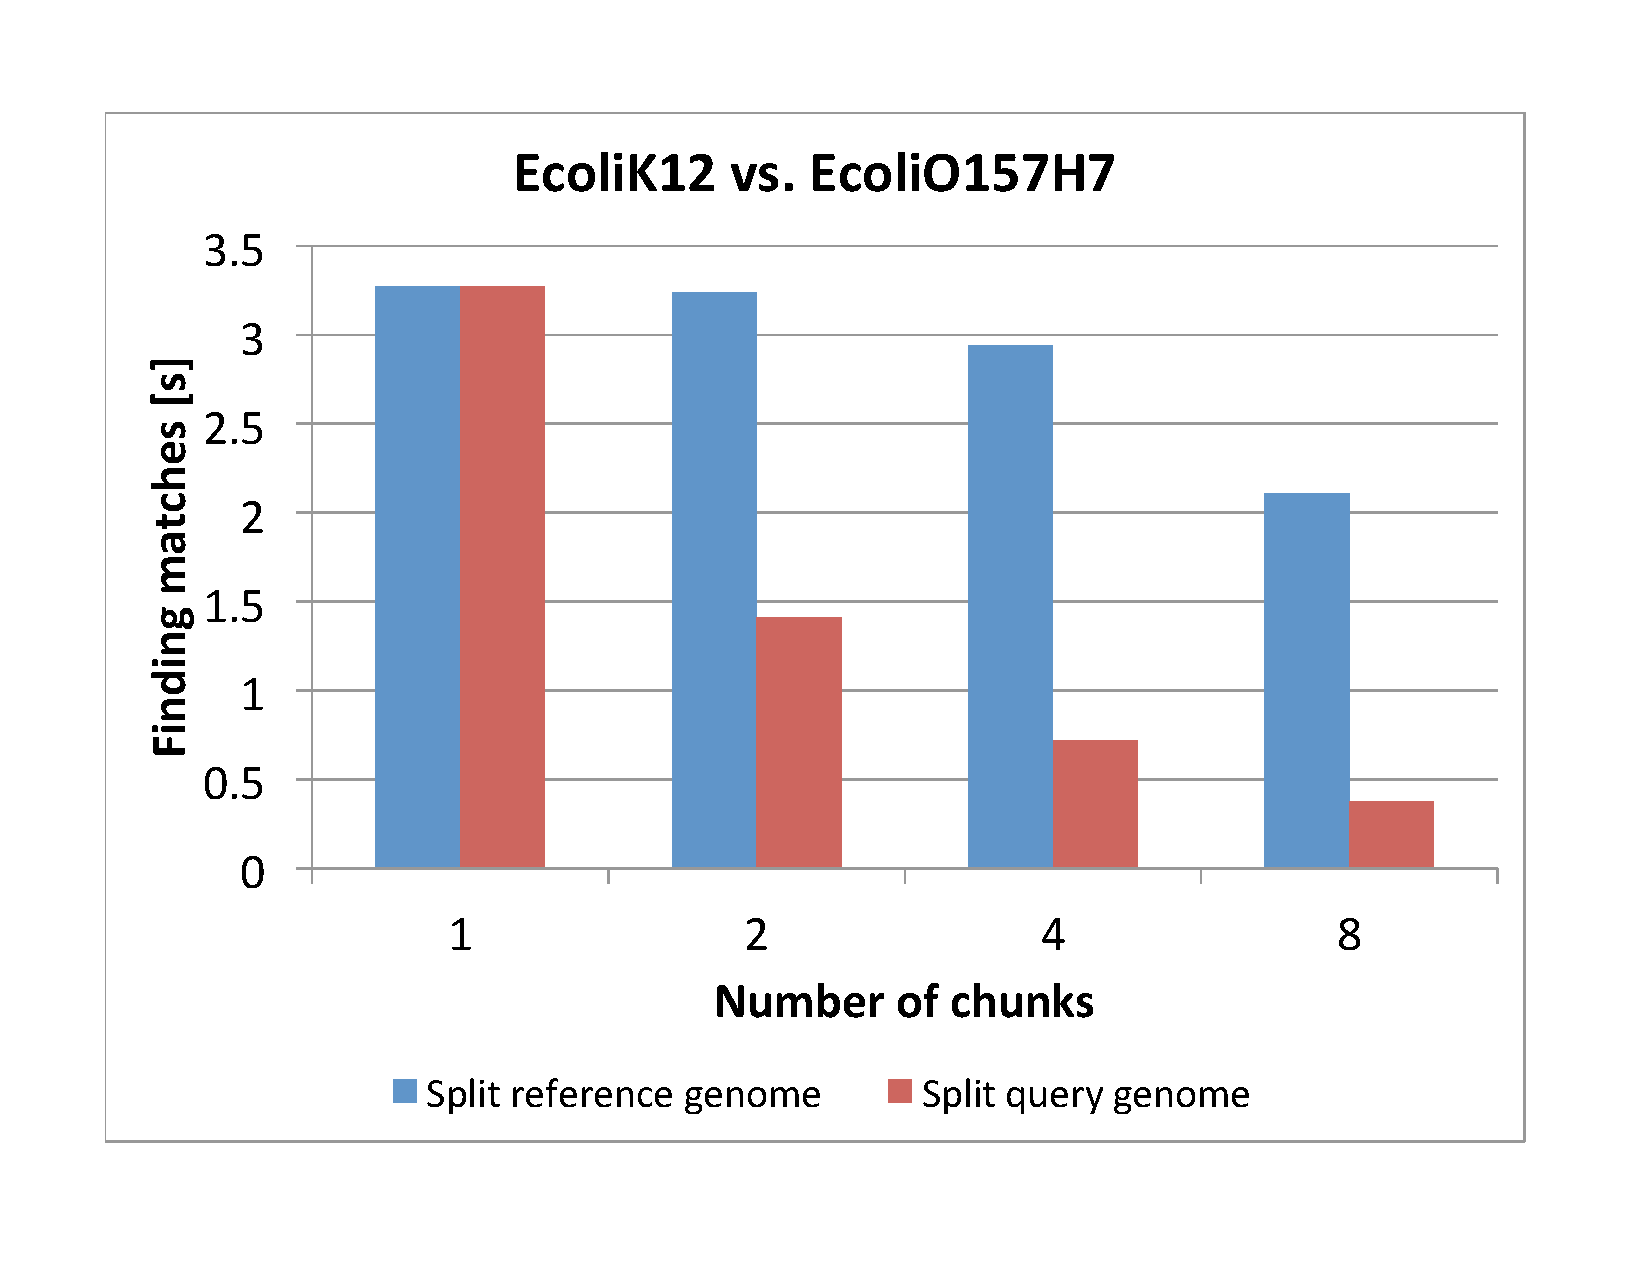
\includegraphics[scale=0.4]{ecoli2012.pdf} 
   \caption{Búsqueda de MEMs para el genoma Ecoli de longitud mínima 20.} 
   \label{fig:ecoliFind} 
 \end{figure}
   \begin{figure}[h] 
   \centering 
   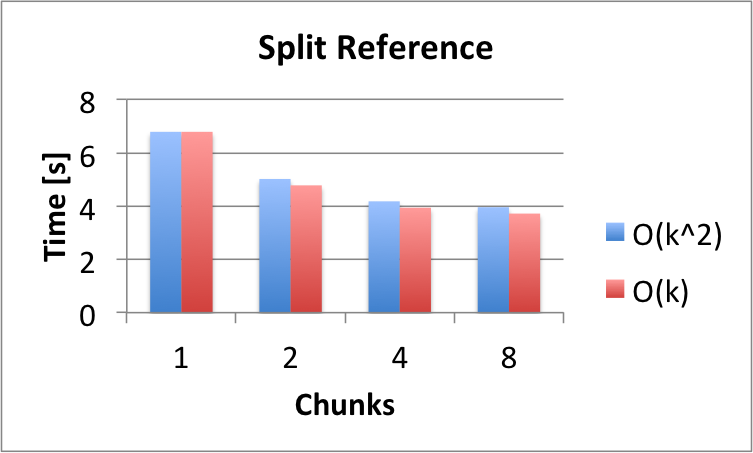
\includegraphics[scale=0.7]{ex3.png} 
   \caption{Evaluación de algoritmo de obtención de lista de MEMs global para el genoma Ecoli.} 
   \label{fig:ecoliMEMR} 
 \end{figure}
   \begin{figure}[h] 
   \centering 
   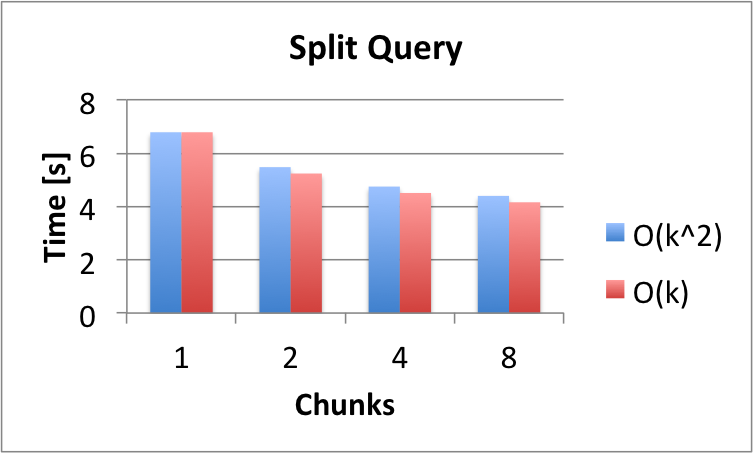
\includegraphics[scale=0.7]{ex6.png} 
   \caption{Evaluación de algoritmo de obtención de lista de MEMs global para el genoma Ecoli.} 
   \label{fig:ecoliMEMQ} 
 \end{figure}
\indent
Un segundo experimento se llevo a cabo evaluando la viabilidad de la propuesta descrita utilizando el cromosoma 19 del homo sapiens y del chimpanc\'e. La búsqueda de MEMs de longitud mínima de 2000 se muestra en la figura \ref{fig:hspanFind} y en la figura \ref{fig:hspanMEMGlobal} se muestra el tiempo de cómputo para la fase final.\\
   \begin{figure}[h] 
   \centering 
   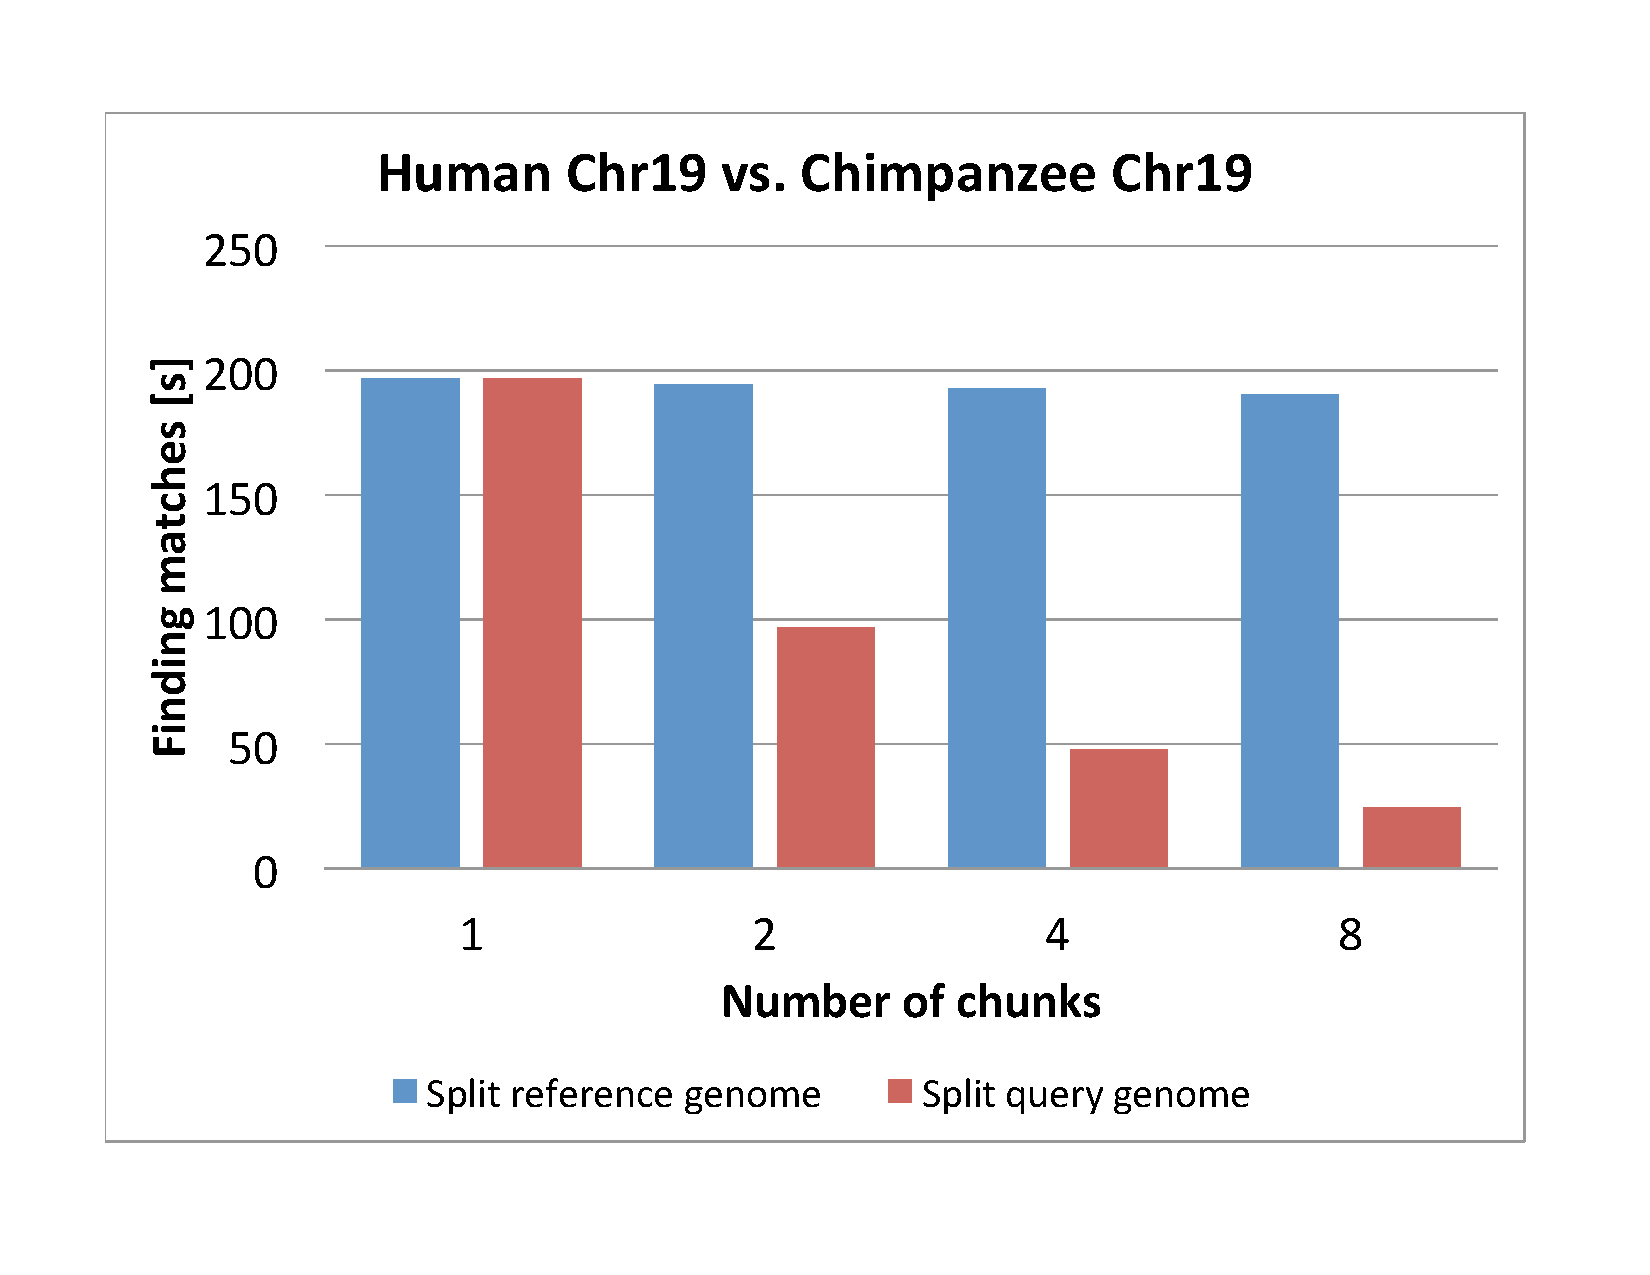
\includegraphics[scale=0.4]{hspan.pdf} 
   \caption{Búsqueda de MEMs para el cromosoma 19 del homo sapiens y el chimpanc\'e de longitud mínima 2000.} 
   \label{fig:hspanFind} 
 \end{figure}
   \begin{figure}[h] 
   \centering 
   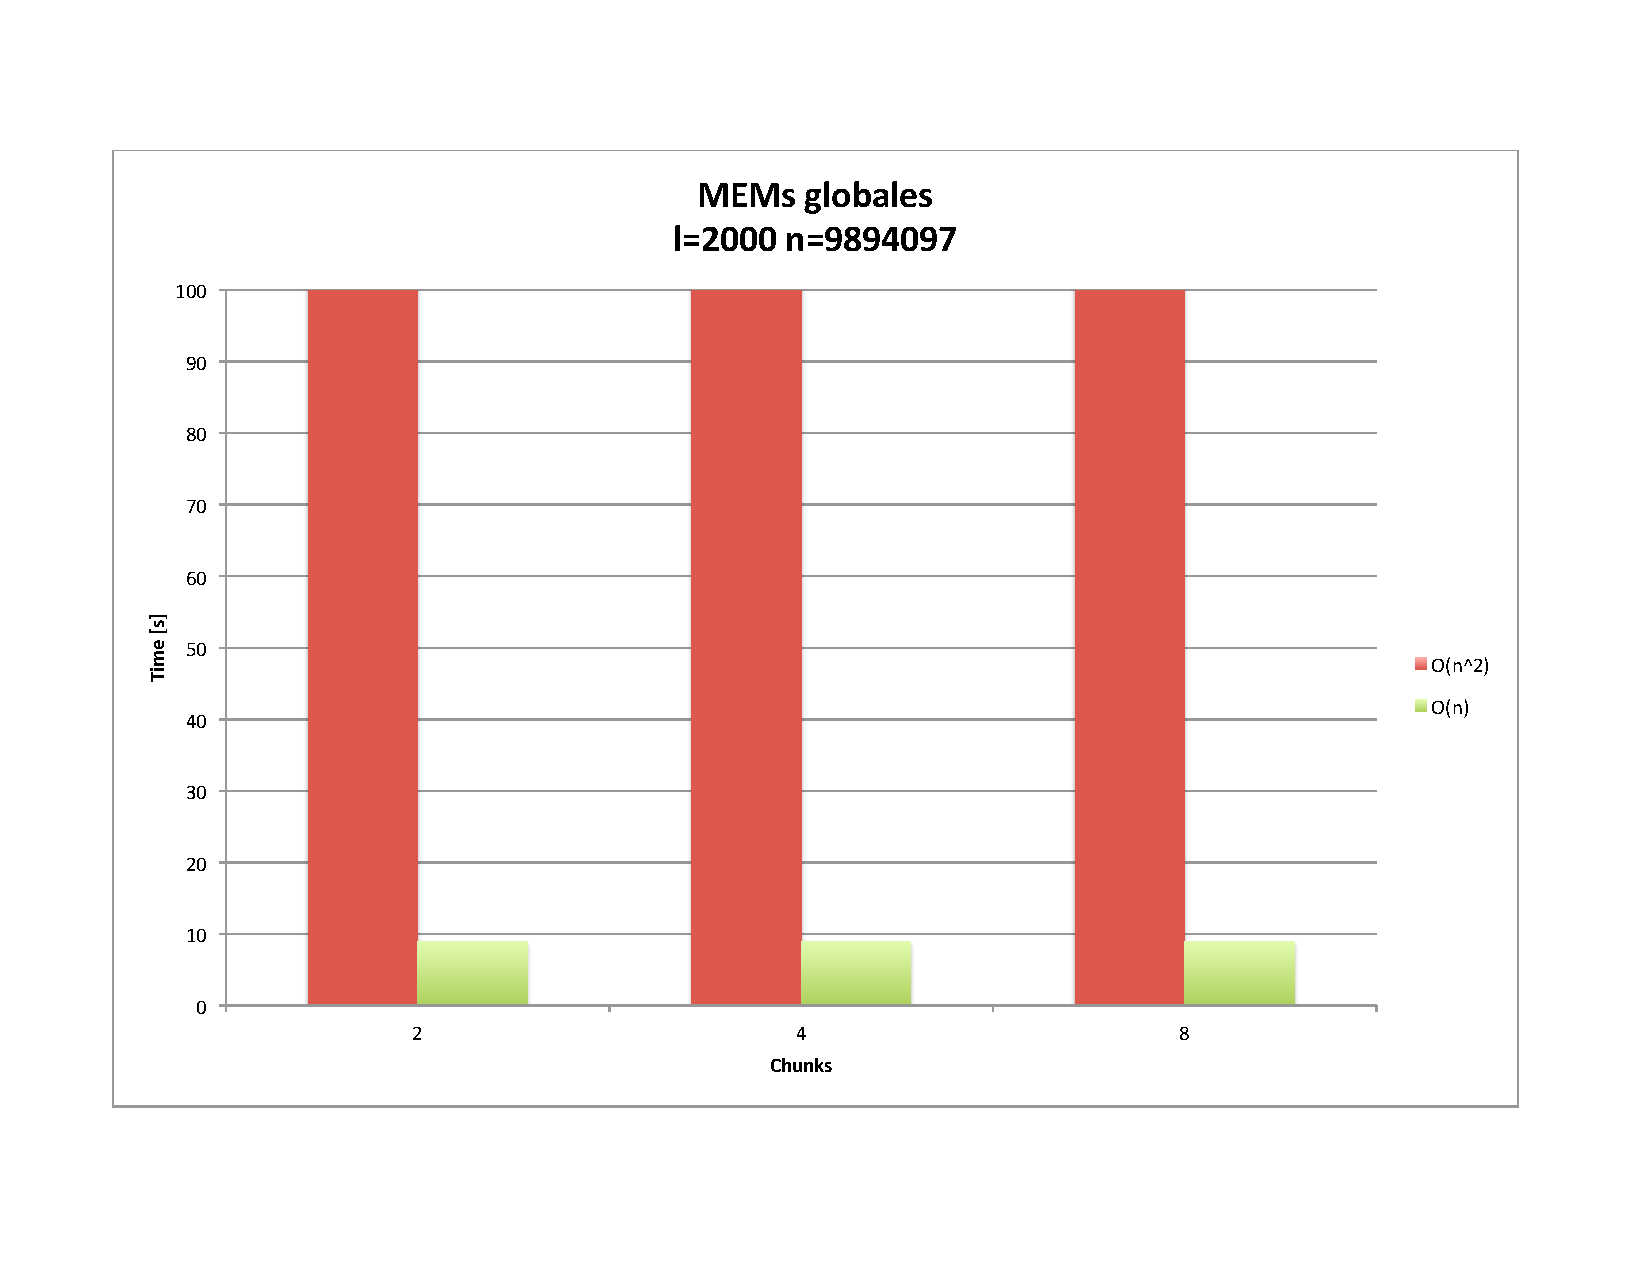
\includegraphics[scale=0.4]{hspanMEMGlobal.pdf} 
   \caption{Evaluación de algoritmo de obtención de lista de MEMs global para el cromosoma 19 del homo sapiens y el chimpanc\'e.} 
   \label{fig:hspanMEMGlobal} 
 \end{figure}
Un detalle importante de resaltar de la mejora realizada al algoritmo simple es la reducción de tiempo obtenido ya que el algoritmo simple tuvo un tiempo de ejecución de más de 7 horas. La mejora en el algoritmo de mezcla de las listas parciales de MEMs en una lista global de MEMs es debido a que el algoritmo simple era muy lento debido a su complejidad computacional $O(g^2)$, donde $g$ es la lista total de MEMs.\\
El primer algoritmo simple realizaba la comparación de cada MEM contra toda la lista de MEMs para determinar si estaba contenido o no por otro MEM. La segunda versión propuesta permite realizar la mezcla de MEMs parciales considerando solo la región en la que se podrían encontrar MEMs cubiertos por un MEM mayor. Está mejora ha permitido reducir el tiempo de cómputo y garantizar que la última fase de esta primera aproximación de paralelización del alineamiento de genomas no se vea afectado por la última fase incluida en la figura \ref{fig:algo}.
\subsection{Búsqueda distribuida de coincidencias exactas: árbol de sufijos distribuido}
\indent
El problema de mejorar el tiempo de cómputo de las búsquedas de coincidencias 
exactas nos da una oportunidad de utilizar el HPC para reducir el
tiempo de procesamiento. Se propone modificar la estructura de datos utilizada en 
MUMmer (árbol de sufijos) para mejorar las búsquedas de coincidencias exactas entre
un genoma de referencia y uno de consulta dada una longitud mínima de coincidencia,
considerando un uso eficiente de los recursos. Para 
ello se tomarán en cuenta los siguientes parámetros: 
\begin{itemize}
\item Optimizar el número de operaciones en la búsqueda de MEMs.
\item Tamaño del genoma de referencia y consulta.
\item Memoria principal disponible en cada nodo de cómputo.
%\item Búsqueda distribuida de coincidencias exactas.
\end{itemize}
\indent
Basado en dichos parámetros se distribuirá el árbol de sufijos en subárboles, 
ver Figura \ref{fig:estructura}. Dicha aproximación ha sido llevada a cabo de distintas maneras por \cite{Mansour2012}, 
\cite{Japp2004}, \cite{Ghoting2010} y \cite{Sadakane}.
 Los subárboles aprovecharán una característica
de la búsqueda de coincidencias: la frecuencia de prefijos en los sufijos del genoma de referencia.\\ 
\begin{figure}[h]
\begin{center}
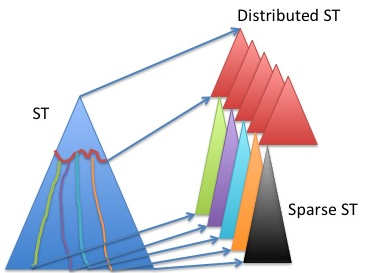
\includegraphics[scale=0.8]{distributed.png}
\caption{Árbol de sufijos distribuido.}
\label{fig:estructura}
\end{center}
\end{figure}
\indent
Para definir formalmente el árbol de sufijos distribuido es necesario mostrar
algunos conceptos, extraídos de \cite{Clifford2005} y \cite{Ghoting2010}. 
\begin{mydef}
  Si $t=uvw$ entonces $u$ es un \textit{prefijo} y $w$ es un \textit{sufijo}
de $t$.
\end{mydef}
\indent
Un sufijo de $t$ se repite si ocurre al menos una vez como una subcadena no sufijo de $t$.
Además requerimos especificar que sufijos de $t$ se incluyen en un subárbol de sufijos. Esto
se hace considerando un prefijo de longitud variable $z$, y el conjunto de prefijos de longitud variable representan 
los subárboles que se almacenan en cada uno de los nodos de cómputo del clúster multicore. El conjunto de prefijos de longitud variable es una idea ya propuesta en \cite{Ghoting2010} que consiste en encontrar la frecuencia de prefijos que cumplen la ecuación \ref{eq:fp}, en la que $f(p)$ es la frecuencia del prefijo $p$, $MTS$ es el tamaño máximo del árbol de sufijos y $NS$ es el tamaño del nodo de un árbol de sufijos en bytes. El factor de 2 es debido a que podemos tener a lo sumo $f(p)$ nodos internos y $f(p)$ nodos hojas.
\begin{center}
\begin{myeq}[!ht]
\begin{equation}
f(p)\le \frac{MTS}{2*NS}
\end{equation}
\caption{Ecuación para el cálculo de prefijos de longitud variable.}
\end{myeq}
\label{eq:fp}
\end{center}
Para generar el árbol de sufijos distribuido DST:
\begin{enumerate}
\item Construir el árbol de sufijos entero en tiempo lineal.
\item Generar el conjunto de prefijos de longitud variable que serán la raíz de cada SST.
\item Para cada prefijo de longitud variable
\begin{enumerate}
\item Extraer el subárbol debajo de ese prefijo, ese subárbol se convierte en el SST.
\item Generar la tabla de direccionamiento de los enlaces de sufijos que apuntan hacia nodos que están fuera del SST. 
\end{enumerate}
\item Refinar la tabla de direccionamiento de los enlaces de sufijos distribuidos con el identificador del SST al que corresponde el nodo hacia el cual apunta.
\end{enumerate}
\indent
El algoritmo resultante usa el espacio en cada nodo que es proporcional al tamaño del SST construido. La generación de los SSTs obliga a contar con un esquema de enlaces de sufijos que apuntan hacia nodos que no están dentro del SST recien creado. Este esquema de enlaces de sufijos distribuido será almacenado en cada uno de los SSTs generados.
\subsection{Importancia del enlace de sufijo}
\indent
Los enlaces de sufijos juegan un rol crítico en la construcción lineal de árboles de sufijos y en su
recorrido.
\begin{mydef}
  Si hay un nodo v en el árbol de sufijos con la etiqueta $c\alpha$, donde c es un carácter y $alpha$
  es una cadena (no vacía), entonces el enlace de sufijo de v apunta a s(v), que es un nodo con la
  etiqueta $\alpha$. Si $\alpha$ está vacío, entonces el enlace de sufijo de v, por ejemplo s(v) es la
  raíz. 
\end{mydef}
\indent
Los enlaces de sufijo existen para cada nodo interno (no hoja) de un árbol de sufijo. Siguiendo un 
enlace de sufijo, se puede saltar de un sufijo a otro, cada sufijo iniciando exactamente un carácter
siguiente del primer carácter de su sufijo precedente. De tal manera que usando \textbf{enlaces de sufijos} es
posible obtener un \textbf{algoritmo lineal para la búsqueda de coincidencias exactas máximas}. Esto es porque
los enlaces de sufijos hacen un seguimiento de que o cuanto de la cadena ha coincidido hasta ahora.
Cuando encontramos una discrepancia, podemos saltar a lo largo del enlace de sufijo para 
ver si hay cualquier coincidencia después en la referencia y en la consulta.\\
\indent
La creación de un DST genera un nuevo problema a resolver, los enlaces de sufijos. Esto es, al construir árboles dispersos SST puede ocurrir que existan enlaces de sufijos que apunten a nodos de otro árbol SST. Para ello es necesario contar con algun esquema que permite seguir el nuevo enlace de sufijo distribuido. Si el número de enlaces de sufijos distribuido de un SST es muy grande pueden ocurrir problemas de sobrecarga de procesamiento en algunos SSTs. Adicionalmente puede trasladar nuestro problema de procesamiento a uno de comunicaciones en el que se tendría que lidiar con el uso de los enlaces de sufijos distribuido.\\
\indent
La solución es contar con un esquema que permita la utilización de enlaces de sufijos distribuido:
\begin{enumerate}
\item Tabla de búsqueda directa del nodo al que apunta el enlace de sufijo distribuido, compartido por todos los SSTs.
\item Sistema de cola para el procesamiento de las peticiones de búsqueda en el SST hacia el cual apunta el enlace de sufijo distribuido.
\end{enumerate}
\indent
Mediante la organización del nuevo árbol de sufijos distribuido de esta manera, 
podemos realizar búsquedas de coincidencias exactas máximas de forma distribuida. Al
utilizar una búsqueda distribuida es posible mejorar el tiempo de cómputo de 
las búsquedas exactas. Se requiere que el tiempo de cómputo sea menor que el 
mostrado por propuestas existentes en el estado del arte.\\
\subsection{Evaluación experimental}
\indent
Los experimentos realizados se ejecutaron en el siguiente ambiente de pruebas:
\begin{enumerate}
\item GCC 4.6.3
\item MUMmer 3.23
\item SparseHash 2.0.2-1
\item Intel(R) Core(TM)2 Duo CPU     E8400  @ 3.00GHz
\item RAM 6GB
\end{enumerate}
\indent
Los genomas utilizados en las pruebas fueron:
\begin{itemize}
\item Genoma humano (2,96Gbp).
\item Cromosoma 2 humano (238,6Mbp).
\item Cromosoma 1 chimpancé (232,7Mbp).
\item EcoliK12 (4,6Mbp).
\item EcoliO157H7 (5,3Mbp).
\end{itemize}
\indent
El primer elemento a evaluar fue la utilización de los enlaces de sufijos al buscar MEMs de diferentes longitudes. Este experimento se realiza para el cromosoma 2 del ser humano como referencia y el cromosoma 1 del chimpancé como consulta. La búsqueda a realizar es de MEM. Se evalúan dos mecanismos de búsqueda de MEMs:
\begin{itemize}
\item Cada sufijo inicia la búsqueda desde la raíz.
\item Cada sufijo utiliza el enlace de sufijo.
\end{itemize}
\indent
En la figura \ref{fig:sl-nosl} se muestra que para diferentes longitudes de MEMs y se comprueba que la ganancia en tiempo de cómputo es siempre mayor al utilizar los enlaces de sufijos que si no se utilizarán. Esta mejora se explica porque al utilizar un enlace de sufijo se evita una comparación cada que se utiliza el enlace de sufijo.\\
\begin{figure}[h]
\begin{center}
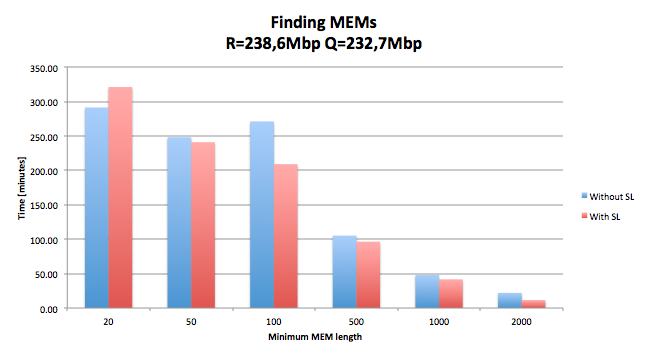
\includegraphics[scale=0.4]{sl-nosl.png}
\caption{Comparación de búsqueda de MEMs con y sin utilización de enlaces de sufijos.}
\label{fig:sl-nosl}
\end{center}
\end{figure}
El tiempo de procesamiento también se ve afectado, evidentemente por la cantidad de MEMs encontrados, como se muestra en la figura \ref{fig:mems}.\\
\begin{figure}[h]
\begin{center}
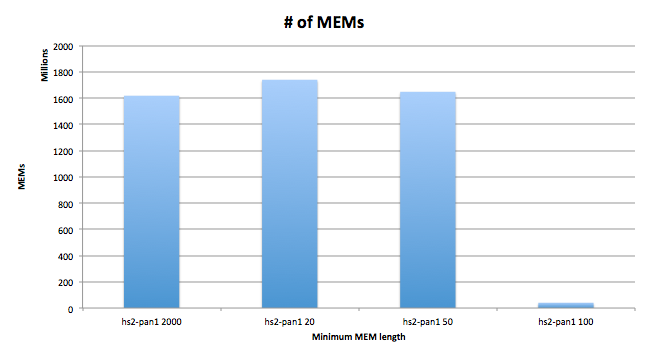
\includegraphics[scale=0.4]{mems.png}
\caption{Conjunto de MEMs encontrados para distintos tamaños mínimos de longitud.}
\label{fig:mems}
\end{center}
\end{figure}
\indent
Una vez que se ha comprobado la efectividad de los enlaces de sufijos se procede a evaluar como son accesados estos enlaces de sufijos y en que zonas del árbol se encuentran. Esto se hace con el fin de evaluar como se verá afectado la búsqueda de MEMs al hacer la división vertical del árbol de sufijos en nuestra propuesta.\\
\indent
Para ello se realizó la búsqueda de MEMs con el genoma de referencia EcoliK12 y con el genoma de consulta EcoliO157H7 con una longitud mínima de 20 de MEM. En la figura \ref{fig:use-sl} se muestra que la longitud mínima de MEM restringe la profundidad del árbol en el cual los enlaces de sufijos son utilizados.\\
\begin{figure}[h]
\begin{center}
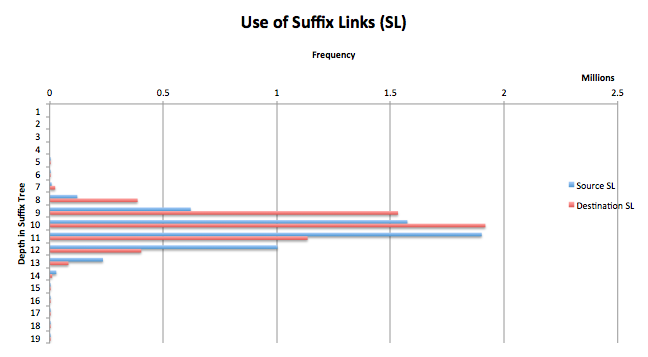
\includegraphics[scale=0.4]{use-sl.png}
\caption{Frecuencia de uso de los enlaces de sufijos al buscar MEMs de longitud mínima de 20bp.}
\label{fig:use-sl}
\end{center}
\end{figure}
\indent
Una posible mejora de optimización consistiría en mejorar la localidad de los nodos que se encuentran en los niveles de profundidad de 8 a 12 que son en donde se utilizan los enlaces de sufijos con mayor frecuencia. Esta posible heurística estaría basada en la longitud mínima de MEM a buscar y que depende del usuario.\\
\indent
Una vez que se ha evaluado la importancia del enlace de sufijo en un árbol de sufijos para la búsqueda de coincidencias exactas máximas se procede a evaluar experimentalmente la propuesta de distribución del árbol de sufijos. Se debe de mantener el enlace de sufijo al hacer la distribución del árbol debido a que esto nos garantiza la complejidad lineal de la búsqueda de MEMs.\\
\indent
El primer paso es determinar el conjunto de prefijos de longitud variable necesario para distribuir el árbol de sufijos. Es por ello que se realizó un experimento para ubicar la longitud necesaria para la elección de los prefijos.\\
\indent 
Al utilizar prefijos de longitud variable es posible tener árboles de sufijos dispersos balanceados debido a que se podrían agrupar aquellos prefijos con mayor frecuencia
de ocurrencia. Es por ello que debemos encontrar un conjunto valido de prefijos para dividir el árbol de sufijos en árboles de sufijos dispersos con el requerimiento de que puedan construirse en memoria principal.\\
\begin{mydef}
Sea $f(p)$ el número de veces que un prefijo ocurre en el genoma de referencia $R$. Sea $MTS$ (tamaño máximo del árbol de sufijos) la cantidad
máxima de espacio de memoria en bytes que puede ser reservado al árbol de sufijos durante la construcción del árbol. 
Sea $NS$ el tamaño de un nodo del árbol de sufijos en bytes.
El objetivo es encontrar un conjunto de prefijos de longitud variable en $R$, tal que $\forall p \epsilon R, f(p)<\frac{MSSTS}{2*NS}$.
\end{mydef}
\indent
Una vez definido el conjunto de prefijos se procede a la construcción del árbol de sufijos disperso. Para ello se ubican en cada
árbol de sufijos disperso el prefijo de longitud variable que será la raíz de cada árbol de sufijos disperso. Una vez 
definido el conjunto de prefijos se procede a la división del árbol de sufijos para obtener el árbol de sufijos disperso. Finalmente se genera la tabla de enlaces de sufijos distribuido correspondiente a cada árbol de sufijos disperso.\\
\indent
Para demostrar como la creación de los prefijos de longitud variable permiten generar árboles de sufijos dispersos, se muestra la frecuencia de prefijos para el genoma humano en las figuras \ref{fig:human-freq2} y \ref{fig:human-freq3}.\\
\begin{figure}[!ht]
\begin{minipage}[b]{0.5\linewidth}
\centering
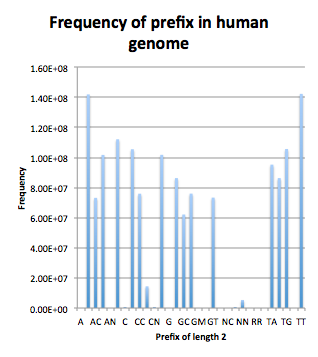
\includegraphics[scale=0.6]{human-freq2.png}
\caption{Frecuencia prefijos de longitud variable en genoma humano.}
\label{fig:human-freq2}
\end{minipage}
\begin{minipage}[b]{0.5\linewidth}
\centering
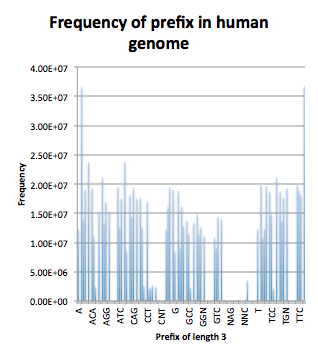
\includegraphics[scale=0.6]{human-freq3.png}
\caption{Frecuencia prefijos de longitud variable en genoma humano.}
\label{fig:human-freq3}
\end{minipage}
\end{figure}
\indent
Si definimos $F_{m}=\frac{MTS}{2*NS}$ entonces de las figuras \ref{fig:human-freq2} y \ref{fig:human-freq3} se obtendrían las raíces de los árboles de sufijos dispersos que son menores que el valor $F_{m}$. Si $F_{m}$ es igual a 1.2\e{8} entonces de la figura \ref{fig:human-freq2} se muestra que se debe de extender los prefijos AA y TT con una longitud mayor hasta que se cumpla que sea menor que $F_{m}$.\\
\indent
Para un genoma real se evalúa la creación del árbol de sufijos distribuido. Con el genoma EcoliK12 se procede a generar el árbol de sufijos distribuido. Se toma en consideración que $F_{m}=150K$, se recorre el genoma de referencia para encontrar el conjunto de prefijos de longitud variable que cumplen la ecuación \ref{eq:fp}. El resultado de este proceso se muestra en las figuras \ref{fig:table-freq2} y \ref{fig:table-freq3}.\\
\begin{figure}[!ht]
\begin{minipage}[b]{0.5\linewidth}
\centering
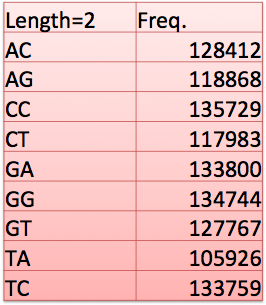
\includegraphics[scale=0.4]{table-freq2.png}
\caption{Frecuencia prefijos de longitud variable en genoma EcoliK12.}
\label{fig:table-freq2}
\end{minipage}
\begin{minipage}[b]{0.5\linewidth}
\centering
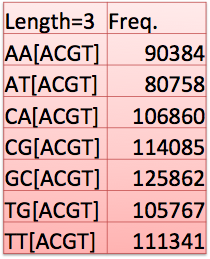
\includegraphics[scale=0.4]{table-freq3.png}
\caption{Frecuencia prefijos de longitud variable en genoma EcoliK12.}
\label{fig:table-freq3}
\end{minipage}
\end{figure}
El siguiente paso es determinar los enlaces de sufijos distribuidos para cada uno de los árboles de sufijos dispersos creados a partir del conjunto de prefijos de longitud variable. En las figuras \ref{fig:dsl1} y \ref{fig:dsl2} se muestra que el porcentaje de enlaces de sufijos distribuido es inferior 1\%.\\
\begin{figure}[!ht]
\begin{minipage}[b]{0.5\linewidth}
\centering
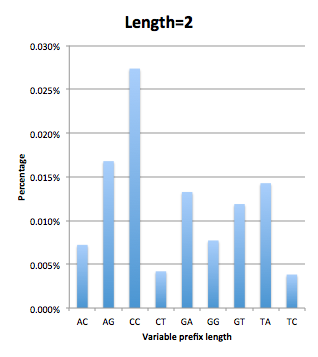
\includegraphics[scale=0.4]{dsl1.png}
\caption{Enlaces de sufijo distribuidos para genoma EcoliK12.}
\label{fig:dsl1}
\end{minipage}
\begin{minipage}[b]{0.5\linewidth}
\centering
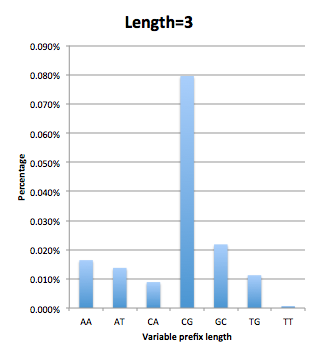
\includegraphics[scale=0.4]{dsl2.png}
\caption{Enlaces de sufijo distribuidos para genoma EcoliK12.}
\label{fig:dsl2}
\end{minipage}
\end{figure}
El resultado del árbol de sufijos distribuido es garantizar la búsqueda de coincidencias exactas máximas en el árbol de sufijos disperso y minizar el traslado de peticiones de búsqueda en árboles externos, las figuras \ref{fig:dsl1} y \ref{fig:dsl2} demuestran que el impacto de distribuir el árbol de sufijos será mínimo.\\
\indent
En la figura \ref{fig:dst} se muestra el árbol de sufijos distribuido con cada uno de los árboles de sufijos disperso. Para una
cadena aacacccacacaccacaaa\$ con sus respectivos nodos raíz etiquetados como $r_{aa}, r_{ac}, r_{ca}, r_{cc}, r_{a\$}$ and $r_{\$}$.
\begin{figure}[h]
\begin{center}
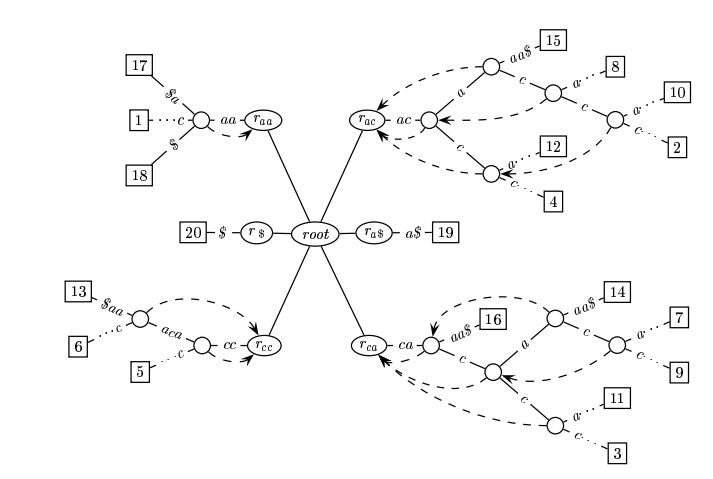
\includegraphics[scale=0.4]{dst2.png}
\caption{Árbol de sufijos distribuido para la cadena: aacacccacacaccacaaa\$.}
\label{fig:dst}
\end{center}
\end{figure}
Una característica que el árbol de sufijos distribuido tiene es que únicamente mantiene los enlaces de sufijos que pertenecen al 
árbol de sufijos disperso. Aquellos enlaces de sufijos que apunten a otros nodos que no están en el árbol de sufijos disperso
son agregados a la tabla de enlaces de sufijos distribuidos.\\
Como se mencionó anteriormente el enlace de sufijo no solo permite la construcción en tiempo lineal del árbol de sufijos sino
que hace que las búsquedas de coincidencias sean tambi\'en lineales. En consecuencia surge ahora un nuevo problema al proponer
esta estructura de datos modificada:\\
\begin{center}
  ¿Es posible mantener la complejidad de búsqueda de coincidencias en un árbol de sufijos $O(m+k)$, en donde $m$ es la
  longitud de la secuencia de consulta y $k$ es el número de ocurrencias al utilizar un árbol de sufijos distribuido?
\end{center}
\subsection{Búsqueda de coincidencias exactas en un DST}
El propósito de adaptar una estructura de datos como el árbol de sufijos es lograr reducir el tiempo de búsqueda de coincidencias
exactas. Para ello se propone una primera aproximación a la búsqueda de coincidencias exactas máximas en un árbol de sufijos 
distribuido.\\
La idea general se basa en dividir la secuencia de consulta en segmentos y asignar la búsqueda de cada sufijo dentro de cada
segmento en el árbol de sufijos disperso correspondiente. La búsqueda de coincidencias exactas se realiza de manera paralela en el árbol de sufijos disperso y 
posteriormente determina las posiciones en las cuales se encuentran las coincidencias. Al evaluar el siguiente sufijo pueden
ocurrir dos casos:
\begin{enumerate}
  \item El siguiente sufijo se encuentra en el mismo árbol de sufijos disperso. La búsqueda continúa de manera local.
  \item La búsqueda del siguiente sufijo se realiza en otro árbol de sufijos disperso.
\end{enumerate}
El segundo caso es de especial relevancia ya que implica el proponer una estrategia de búsqueda del árbol de sufijos disperso
en donde se debe realizar la búsqueda y adicionalmente continuar la búsqueda en ese árbol.\\
Para solucionar este caso, se propone el envío de la petición de búsqueda del sufijo en el árbol correspondiente utilizando la tabla de enlaces de sufijos distribuido. El árbol que recibe la petición la encola en la lista de sufijos que tiene que procesar y 
resuelve la búsqueda de coincidencias exactas máximas del sufijo que se le ha asignado.\\
En la figura \ref{fig:dst_search} se muestra de manera gráfica la búsqueda de coincidencias exactas para una secuencia de consulta,
la división en segmentos de la misma y la búsqueda del primer sufijo de cada segmento en el árbol de sufijos distribuido.
\begin{figure}[h] 
\begin{center}
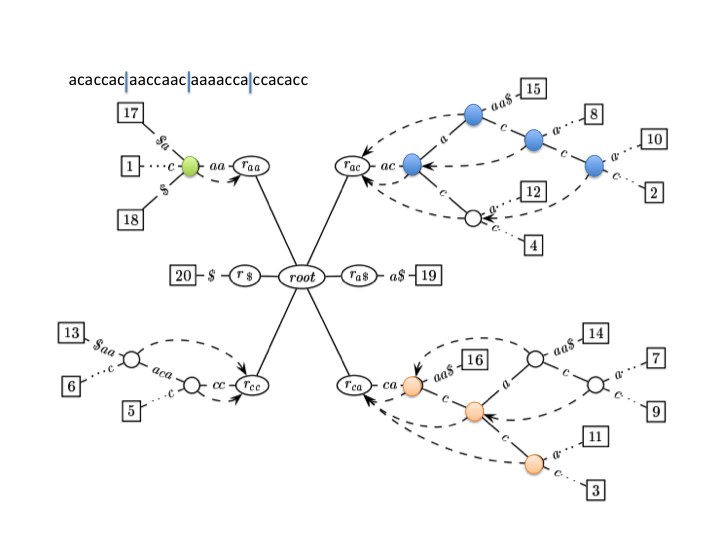
\includegraphics[scale=0.4]{dst_search.png}
\caption{Búsqueda de coincidencias exactas máximas en un árbol de sufijos distribuido.}
\label{fig:dst_search}
\end{center}
\end{figure}

\section{Publicaciones}
\noindent
Ninguna.
\section{Seguimiento}
En el primer año se ha cumplido con la adaptación de una estructura de datos que permita su utilización
en el alineamiento de datos biológicos a gran escala. Dicha estructura será la base del desarrollo de MUMmer en HPC.
La estructura es capaz de manejar grandes volúmenes de datos y se pueden realizar operaciones de consulta sobre ella.
\section{Planificación}
En el segundo año se realizará el diseño y evaluación experimental de un algoritmo paralelo y distribuido de búsquedas de 
coincidencias exactas máximas. Para ello se aprovechará la estructura de datos diseñada en el primer año. Se adaptará este
algoritmo a la aplicación MUMmer para su ejecución en entornos de HPC.
En el tercer año se refinará la ejecución de MUMmer en entornos de HPC. Se tomará como base el programa original, MUMmer, y 
se realizarán las modificaciones pertinentes para mejorar la fase de agrupamientos de MUMs y MEMs. Estancia en otra unidad 
de investigación, EMBL Heidelberg Alemania. Adaptar la propuesta de búsqueda distribuida de coincidencias exactas desarrollado para su
ejecución en las instalaciones de EMBL. Redactar la tesis doctoral y preparar su defensa.
\section{Análisis de las publicaciones pendientes de publicar}
\noindent
Ninguna.
\section{Publicaciones previstas}
%Asia Pacific Bioinformatics Conference - \href{http://www.apbc2013.org/}{APBC} - Julio 2012 : Una tema de investigación en el congreso es Comparative genomics que forma parte del problema que se está resolviendo, el alineamiento de genomas.\\
IEEE International Symposium on Parallel and Distributed Processing with Applications - \href{http://www.arcos.inf.uc3m.es/ispa12/}{ISPA} - Enero 2013 : La estructura del árbol de sufijos distribuidos forma parte de los temas de investigación en este congreso.\\
International Conference on Parallel Processing - \href{http://www.grs-sim.de/news-events/news-archive/euro-par-2013.html}{Euro-Par} - Febrero 2013 : El algoritmo de búsqueda de coincidencias exactas máximas distribuida forma parte de los temas aboradados en este congreso.\\
European Symposium on Algorithms - \href{http://esa-symposium.org/}{ESA} - Abril 2013 : El algoritmo de búsqueda distribuida de coincidencias exactas máximas distribuida forma parte de los temas abordados en este congreso.\\
International Symposium on Algorithms and Computation - \href{http://www.is.titech.ac.jp/isaac11/}{ISAAC} - Junio 2013 :  El algoritmo de búsqueda distribuida de coincidencias exactas máximas distribuida forma parte de los temas abordados en este congreso.\\
\section{Conclusiones}
\indent
Durante este primer año de investigación doctoral se ha estudiado y evaluado la estructura de datos utilizada en la aplicación MUMMer.
Se ha mejorado la fase de obtención de la lista final de MEMs reduciendo la complejidad del algoritmo utilizado previamente.
Se han diseñado diferentes experimentos para determinar la mejor manera de dividir dicha estructura y aprovechar la nueva estructura
en entornos de HPC. Se evalúo la utilidad de los enlaces de sufijos en un árbol de sufijos y como se pueden aprovechar para la 
búsqueda de coincidencias exactas máximas.\\
\indent
Se ha adaptado el árbol de sufijos para su ejecución en entornos de HPC y se ha propuesto una solución al problema de  la restricción
de memoria cuando la cadena de referencia crece. La estructura de datos adaptada se ha utilizado para proponer una primera aproximación a la 
solución de mejorar el tiempo de búsqueda de coincidencias exactas máximas.\\
\indent
En el siguiente año se busca determinar si la propuesta de búsqueda de coincidencias exactas máximas en el árbol de sufijos distribuido 
permite mejorar el tiempo de ejecución bajo entornos de HPC. Adicionalmente se tendrán que resolver los siguientes problemas
\begin{itemize}
  \item Política de carga de trabajo para cada árbol de sufijos disperso: garantizar que todas las búsquedas se resuelvan de manera local.
  \item Búsqueda de coincidencias exactas máximas en el árbol de sufijos disperso de forma paralela, es decir, realizar múltiples búsquedas
    para distintos sufijos bajo el paradigma de las arquitecturas multicore. 
\end{itemize}
\bibliographystyle{apalike} 
\bibliography{references}	
\end{document}
